\documentclass[12pt]{article}
\usepackage{amsmath}
\usepackage{graphicx}
\usepackage{float}
\usepackage[utf8]{inputenc}
\usepackage{cite}
\usepackage{setspace}
\usepackage{amsfonts}
\usepackage{mathrsfs}
\usepackage[margin=1.0in]{geometry}
\usepackage{enumitem}
\usepackage{listings}
\usepackage{subfigure}

\numberwithin{equation}{section}

\title{Developing a Numerical Solution to Ferromagnetic Materials}
\author{Elizabeth Drueke}

\begin{document}
\maketitle

\begin{abstract}
Modeling lattice-type structures under the effects of magnetization has been achieved with reasonable accuracy using the Ising model.  In order to accurately describe the larger of these systems, it is important to develop computer algorithms which can do large-scale computations in small amounts of time.  To this end, we develop a Monte Carlo process using the Metropolis Algorithm to study the effects of magnetization on two-dimensional lattice systems of various sizes and at various temperatures, and use the results of this analysis to determine the accuracy of our algorithm.  In partiular, we focus on the effect of various random number generators on the results, to ensure that we are not encountering a strong systematic bias from this source.
\end{abstract}

\section{Introduction}
\label{sec:intro}

To say that magnetism is an important physical phenomenon is a strong understatement.  Magnetism plays a strong role in day to day life on earth.  The earth's magnetic field is perhaps the most stunning example of this.  Caused by the electric fields resulting from the magma under the earth's crust \textbf{http://hyperphysics.phy-astr.gsu.edu/hbase/magnetic/magearth.html}, the earth's magnetic field has been used by explorers for centuries to navigate both on land and sea.  Today, we are still using magnetization to explore the world around us, although in slightly different ways.  For example, magnets are used in some of the largest physics experiments in the world, such as the Large Hadron Collider (LHC), which uses them both as a means of accelerating particles to high energies and as a means of bending charged particles in detectors in an attempt to classify them and thus answer some of the fundamental questions about the universe in which we live.
\par In general, there are three kinds of magnetism: diamagnetism, paramagnetism, and ferromagnetism, which is the subject of this paper.  The types of magnetism are distinguished by the behavior of the spins of atoms within the material being magnetized.  In paramagnets, the spins align parallel to the magnetic field whereas in diamagnets the spins align opposite to the field.  In ferromagnetic material, however, we have the special situation where the material retains its magnetized state even after the polarizing field has been removed.  In this way, ferromagnets may represent a magnetic history of the fields it has encountered. \textbf{cite Griffiths}.  The simplest theoretical model we have to describe ferromagnetism is the Ising model, described in Section~\ref{sec:theory}.  
\par In this paper, we will discuss the Ising model and its importance, and then go into the Monte Carlo algorithm used to do the calculations of various statistical quantities in Section~\ref{sec:algorithm}, taking special note of various benchmarks developed for the case of a $2\times2$ lattice in Section~\ref{subsec:benchmarks}.  Finally, we discuss results of our calculations in Section~\ref{sec:results}.

\section{Theory}
\label{sec:theory}

As mentioned in Section~\ref{sec:intro}, the Ising model is one of the simplest models we have to describe ferromagnetic material.  It does this by expressing the energy in a simple form,
\begin{equation}
\label{eq:isingenergyfull}
E = -J\sum_{\left<kl\right>}^{N}s_{k}s_{l}-B\sum_{k}^{N}s_{k},
\end{equation}
where $s_{k}=\pm1$ is the spin of the $k^{\text{th}}$ lattice point, $J$ is a coupling constant expressing the strength of the interaction between the neighboring spins, $B$ is the externam magnetic field the material is in, and the first sum is taken over nearest neighbors (ie. lattice points directly above, below, to the left, or to the right of each other, assuming periodic boundary conditions).  Because we are working with ferromagnetic materials, which can retain magnetization in the absence of magnetic fields, we can take $B=0$, and so~\eqref{eq:isingenergyfull} becomes
\begin{equation}
\label{eq:isingenergy}
E = -J\sum_{\left<kl\right>}^{N}s_{k}s_{l}.
\end{equation}
\par While~\eqref{eq:isingenergy}~\textbf{cite lecture notes} forms the bulk of the math behind what we will discuss here, it is not the only interesting statistical mechanical quantity we will be interested in.  Thus, before we go too far into things, it may behoove us to discuss briefly concepts such as probabilitiy distributions and specific heat.  Statistical mechanics is a science concerned primarily with the expected behavior exhibited by large groups of interacting objects (spins).  As such, it relies heavily on probability because it quickly becomes unfeasible and, in most cases, impossible, to determine exactly how each individual spin is behaving.  Thus, we are often interested in the expected values of various physical quantities.  In particular, the expected value of some physical quantity $X$ is given by 
\begin{equation}
\label{eq:expvaldef}
\left<X\right>=\sum_{i=1}^{N}X_{i}P_{i},
\end{equation}
where the sum is over all possible states, $X_{i}$ is the value of $X$ in state $i$, and $P_{i}$ is a probability distribution function.  The probability distribution function typically used in statistical mechanics is the Boltzmann distribution, 
\begin{equation}
\label{eq:boltzmann}
P_{i} = \frac{e^{-\frac{E_{i}}{k_{B}T}}}{Z},
\end{equation}
where $E_{i}$ is the energy of state $i$, $k_{B}$ is the Boltzmann constant, $T$ is the temperature, and $Z$ is the partition function, given by
\begin{equation}
\label{eq:partition}
Z=\sum_{i=1}^{N}e^{-\frac{E_{i}}{k_{B}T}}.
\end{equation}

\begin{figure}[ht]
\begin{center}
\subfigure[]{
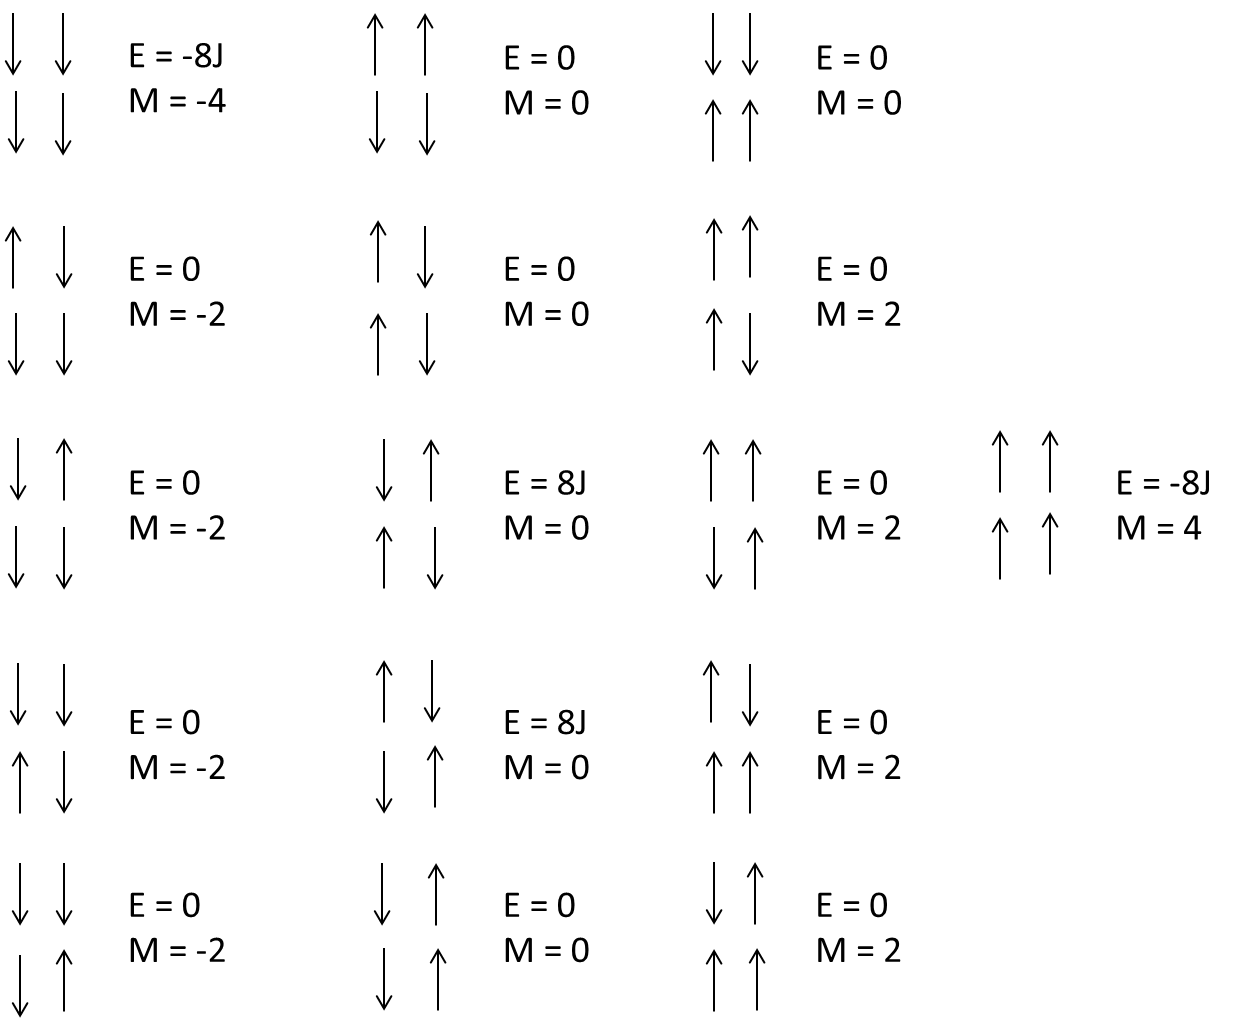
\includegraphics[width=0.6\linewidth]{spin_orientations}
}
\caption{The 16 possible spin orientations, with their energies and magnitizations, for a $2\times2$ lattice.}
\label{fig:spins2x2}
\end{center}
\end{figure}

\par As an example, we might consider a $2\times2$ ferromagnetic lattice.  In order to find any important statistical mechanical quantities, it will be important to determine the partition function.  We note that there are $2^{4}=16$ possible states of this system, as any lattice point can be spin up or spin down.  Already this is quite a few states to look at explicitly individually, but for the purposes of illustration we do so in Fig~\ref{fig:spins2x2}.  We see that there are two states with energy $+8J$, two with energy $-8J$, and 12 with energy $0$.  This yields a partition function of
\begin{equation}
\label{eq:partition2x2}
Z=2e^{-\frac{8J}{k_{B}T}}+2e^{\frac{8J}{k_{B}T}}+12 = 4\cosh{\frac{8J}{k_{B}T}}+12.
\end{equation}
Using~\eqref{eq:expvaldef}, we see also that
\begin{equation}
\label{eq:expe2x2}
\left<E\right> = \frac{1}{Z}\left(16Je^{-\frac{8J}{k_{B}T}}-16Je^{\frac{8J}{k_{B}T}}\right) = \frac{-32J\sinh{\frac{8J}{k_{B}T}}}{Z}.
\end{equation}
\par We are not only interested in the energy, however.  We also want to investigate the magnetization, which is given by
\begin{equation}
\label{eq:mag}
M_{i}=\sum_{i=1}^{N}s_{i}.
\end{equation}
With this simple equation, we can see that the magnetizations for each possible state in the $2\times2$ system are also given in Fig.~\ref{fig:spins2x2} and that
\begin{equation}
\label{eq:expm2x2}
\left<M\right>=0,
\end{equation}
or, perhaps more enlighteningly,
\begin{equation}
\label{eq:expabsm2x2}
\left<\left|M\right|\right> = \frac{1}{Z}\left(8e^{\frac{8J}{k_{B}T}}+4\right).
\end{equation}
\par The final two statistical quantities we will be interested in are the specific heat, given by
\begin{equation}
\label{eq:cvdef}
C_{V} = \frac{1}{k_{B}T^{2}}\left(\left<E^{2}\right>-\left<E\right>^{2}\right)
\end{equation}
and the susceptibility, given by
\begin{equation}
\label{eq:chidef}
\chi = \frac{1}{k_{B}T}\left(\left<M^{2}\right>-\left<M\right>^{2}\right).
\end{equation}
In our $2\times2$ case, we will have
$$
\left<E^{2}\right> = \frac{256J^{2}\cosh{\frac{8J}{k_{B}T}}}{Z}
$$
and
$$
\left<M^{2}\right> = \frac{1}{Z}\left(32e^{\frac{8J}{k_{B}T}}+8\right).
$$
Thus,
\begin{equation}
\label{eq:cv2x2}
C_{V}=\frac{1}{k_{B}T^{2}}\left(\frac{256J^{2}\cosh{\frac{8J}{k_{B}T}}}{Z}-\left(\frac{-32J\sinh{\frac{8J}{k_{B}T}}}{Z}\right)^{2}\right)=\frac{256J^{2}}{k_{B}T^{2}Z}\left(\cosh{\frac{8J}{k_{B}T}}-4\sinh^{2}{\frac{8J}{k_{B}T}}\right)
\end{equation}
and
\begin{equation}
\label{eq:chi2x2}
\chi = \frac{32e^{\frac{8J}{k_{B}T}}+8}{Zk_{B}T}.
\end{equation}

\section{The Algorithm}
\label{sec:algorithm}

For this model, we developed a new class, the \texttt{lattice} class, which directly computes various statistical mechanical quantities for a lattice of a given size and temperature.  In particular, each \texttt{lattice} object has the following objects:
\begin{itemize}
\item \texttt{size}, an \texttt{int} which gives the size of the square lattice (ie. $n$ for an $n\times n$ lattice),
\item \texttt{spins}, a dynamically allocated matrix of the spins in the matrix,
\item \texttt{temp}, a \texttt{double} which gives the temperature of the matrix,
\item \texttt{averages}, a dynamically allocated vector of the averages of $E$, $E^{2}$, $M$, $M^{2}$, and $|M|$,
\item \texttt{MCcycles}, an \texttt{int} which gives the number of Monte Carlo cycles to be used in the calculation,
\item \texttt{CV}, a \texttt{double} of the specific heat,
\item \texttt{chi}, a \texttt{double} of the susceptibility,
\item \texttt{chi\_absm}, a \texttt{double} of the susceptibility calculated from $<|M|>$ rather than $<M>$ (that is, $\chi_{|M|}=<M^{2}>-<|M|>^{2}$),
\item \texttt{accepted}, an \texttt{int} of the number of Monte Carlo events accepted in the calculation, and
\item \texttt{e\_probs}, a \texttt{map} of an energy value to the number of times that energy appears in the calculations.
\end{itemize}
\par The \texttt{lattice} class also has several important functions.  In addition to a default constructor, copy constructor, and  destructor, \texttt{lattice} has a:
\begin{itemize}
\item constructor from a size, temperature, number of Monte Carlo cycles, and the option to start at a lowest-energy state,
\item several "get" functions (eg. \texttt{get\_{E}()}), which returns some statistical mechanical quantities,
\item several "set" function (eg. \texttt{set\_temp(double t)}), which resets and recalculates some variable,
\item \texttt{plot\_eprobs(string name)}, which plots the probability of various energy values $E$ appearing in the calculations, and
\item \texttt{calc\_stat\_quants()}, which is a private function which performs all of the calculations and sets all of the variables as the \texttt{lattice} object is constructed.
\end{itemize} 
\par The Ising model is an excellent example of a physics model which requires the use of Monte Carlo in order to implement on a computer.  The meat of this calculation is performed in the \texttt{calc\_stat\_quants()} function, which is called by all constructors after a random (or not) initial state is set for the lattice.  This function begins by calculating the initial energy with periodic boundary conditions
\begin{verbatim}
  double E=0; double M=0;
  for(int i=0;i<size;i++){
    for(int j=0;j<size;j++){
      M+=spins[i][j];
      E-=spins[i][j]*(spins[(i+size-1)%size][j]+spins[i][(j+size-1)%size]);
    }
  }
\end{verbatim}
Then, it begins the Monte Carlo simulation.  Iterating through integers \texttt{cycle} which are less than the \texttt{MCcycles} parameter, it first randomly changes one of the spins in the lattice:
\begin{verbatim}
    int rando = rand()%(size*size); 
    int ct = 0;
    int therow = 0; int thecol = 0;
    
    for(int i=0;i<size;i++){
      for(int j=0;j<size;j++){
          if(ct==rando){
             spins[i][j]*=-1;
             therow = i;
             thecol = j;
           }
           ct+=1;
        }
      }
\end{verbatim}
It then calculates the change in energy resulting from changing this spin by calling the \texttt{nearest\_neighbors()} function, which    takes in the row and column which were changes as well as the \texttt{spins} matrix and goes through the nearest neighbors of the changed spin to determine what $\Delta E$ should be based on Fig.~\ref{fig:deltaEs}, which shows the only possible five values of $\Delta E$ based on the number of spin-up and spin-down nearest neighbors are around the changed spin.  \texttt{nearest\_neighbors()} returns the $\Delta E$ value as 
\begin{verbatim}
double deltaE = (-4*ups+8)*(spins[row][col]);
return deltaE;
\end{verbatim}

\begin{figure}[ht]
\begin{center}
\subfigure[]{
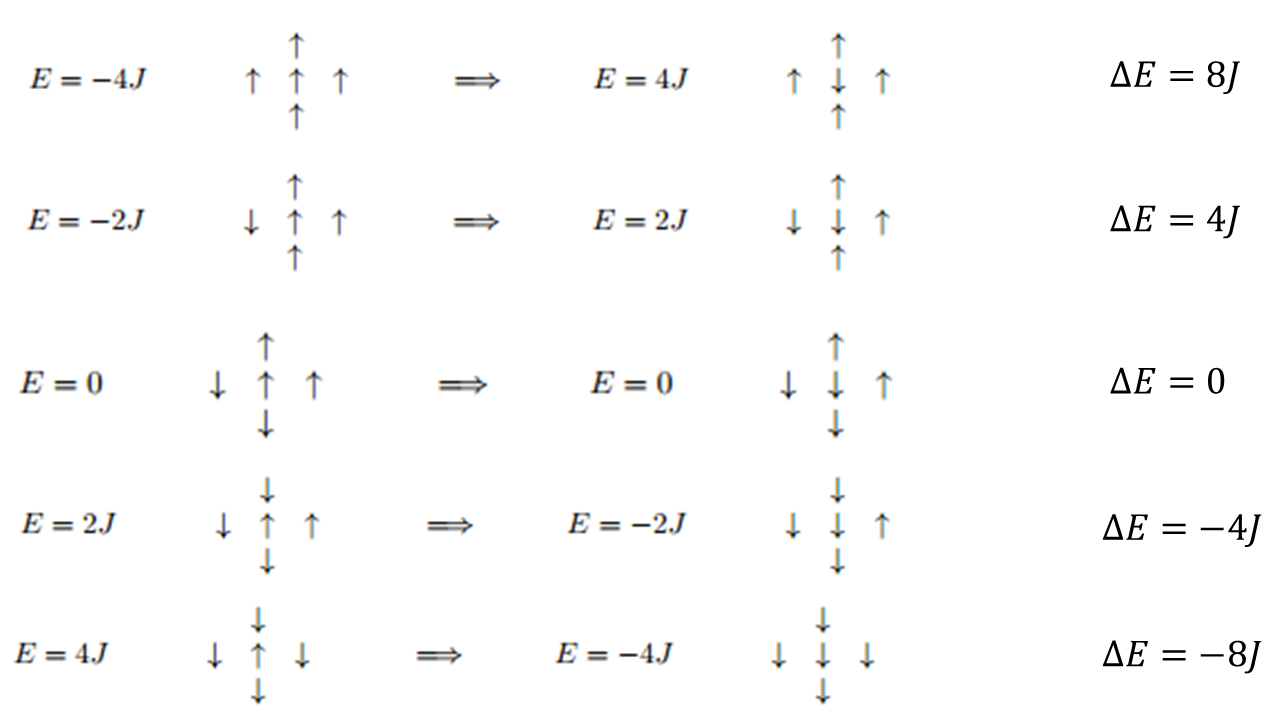
\includegraphics[width=0.6\textwidth]{deltaEs}
}
\caption{The possible values of $\Delta E$ for the $2\times2$ lattice after changing one spin~\textbf{cite lecture notes}.}
\label{fig:deltaEs}
\end{center}
\end{figure}

\par If the change in energy is negative, we generate a random number \texttt{myrand} (in $[0,1]$) and compare it to $w=e^{-\frac{\Delta E}{k_{B}T}}$.  In particular, if $w \leq$ \texttt{myrand}, we keep the change in spin.  However, if $w >$ \texttt{myrand}, we keep the spin matrix as it was before.  That is, 
\begin{verbatim}
    if(deltaE>0){
      double w = exp(-1.0*deltaE/(kB*temp));
      double myrand = (rand()%100000)/100000.0;  
      if(myrand>w){
           spins[therow][thecol]*=-1;
           deltaE=0;
           go = false;
      }
    }

    if(go){
      accepted++;
      M+= 2*spins[therow][thecol];
      E+= deltaE;
    }  
\end{verbatim}
\par Finally, we update the \texttt{averages} vector and \texttt{e\_probs}.  At every Monte Carlo cycle, we add new value of the various statistical quantities to the appropriate component of \texttt{averages} and, after all of the Monte Carlo cycles are through, we divide by \texttt{MCcycles} to get the average value.  Finally, we can calculate our final statistical mechanical quantities:
\begin{verbatim}
  CV = (1.0/(kB*pow(temp,2)))*(averages[1]-pow(averages[0],2));
  chi = (1.0/(kB*temp))*(averages[3]-pow(averages[2],2));
  chi_absm = (1.0/(kB*temp))*(averages[3]-pow(averages[4],2));
\end{verbatim}

\subsection{Benchmarks}
\label{subsec:benchmarks}

To ensure that our algorithm was working properly, we ran a test on the $2\times2$ case discussed in Section~\ref{sec:theory}.  From~\eqref{eq:partition2x2},~\eqref{eq:expe2x2},~\eqref{eq:expm2x2},~\eqref{eq:expabsm2x2},~\eqref{eq:cv2x2}, and~\eqref{eq:chi2x2}, we expect that, for a temperature of $T$ which allows $k_{B}T/J=1$ for coupling $J=1$ (ie. $T=1/k_{B}$), we will have the results listed in Table~\ref{tab:2x2exp}.  The results from the Monte Carlo code are shown in Fig.~\ref{fig:benchmarks} for $<E>$, $<|M|>$, $C_{V}$, and $\chi$.  We see that, in all cases, the simulation models the expected behavior quite well very quickly ($\sim1000$ MC cycles) for $<E>$, $<|M|>$, and $C_{V}$, although it requires significantly more ($\sim200\times10^{3}$) Monte Carlo cycles to achieve a somewhat reliable susceptibility.  For this benchmark, our random number generator used in the Metropolis Algorithm was the standard C++ random number generator seeded with \texttt{time(NULL)} and implemented as
\begin{verbatim}
double myrand = (rand()\%10000)/10000.0;
\end{verbatim}
to ensure that the random variable was in the interval $[0,1]$.

\begin{table}[ht]
\begin{center}
\begin{tabular}{c|c} \hline
Statistical Quantity & $2\times2$ Accepted Value \\ \hline
$Z$ & 5973.917 \\
$\left<E\right> &  -7.984 \\
$\left<\left|M\right|\right> & 3.993 \\
$\left<E^{2}\right> & 63.871 \\
$\left<M^{2}\right> & 15.969 \\
$C_{V}$ & 0.127 \\
$\chi$ & 16.001
\end{tabular}
\caption{The accepted calculated values for the $2\times2$ lattice under the Ising model from the equations derived in Section~\ref{sec:theory}.}
\label{tab:2x2exp}
\end{center}
\end{table}

\begin{figure}[ht]
\begin{center}
\subfigure[]{
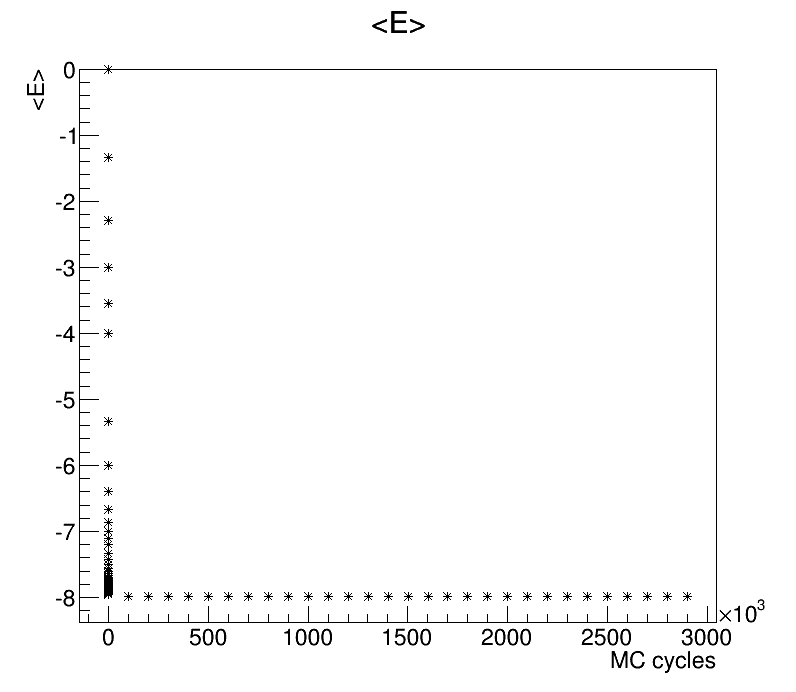
\includegraphics[width=0.3\textwidth]{benchmarks/plots/plots_random_meanE_size2_temp1}
}
\subfigure[]{
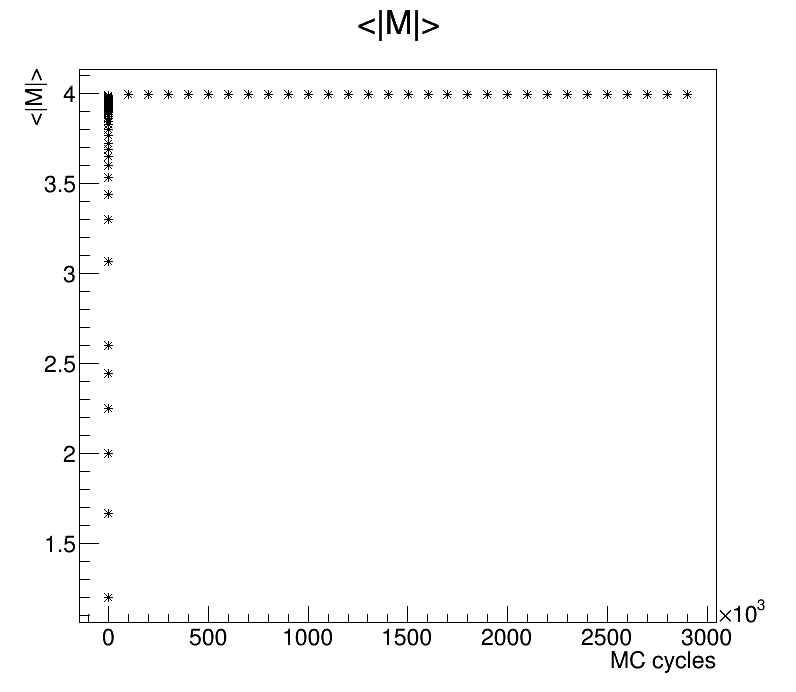
\includegraphics[width=0.3\textwidth]{benchmarks/plots/plots_random_meanAbsM_size2_temp1}
} \\
\subfigure[]{
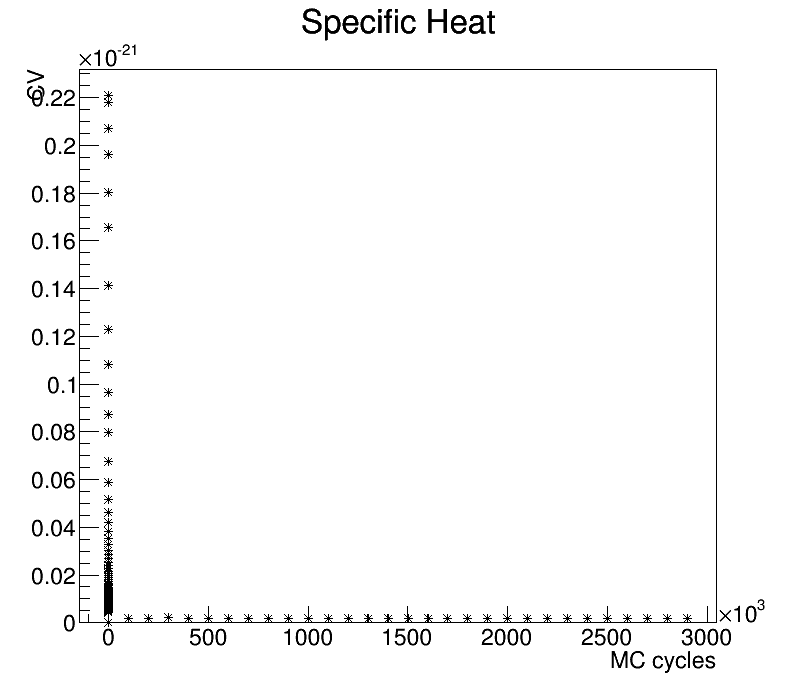
\includegraphics[width=0.3\textwidth]{benchmarks/plots/plots_random_CV_size2_temp1}
}
\subfigure[]{
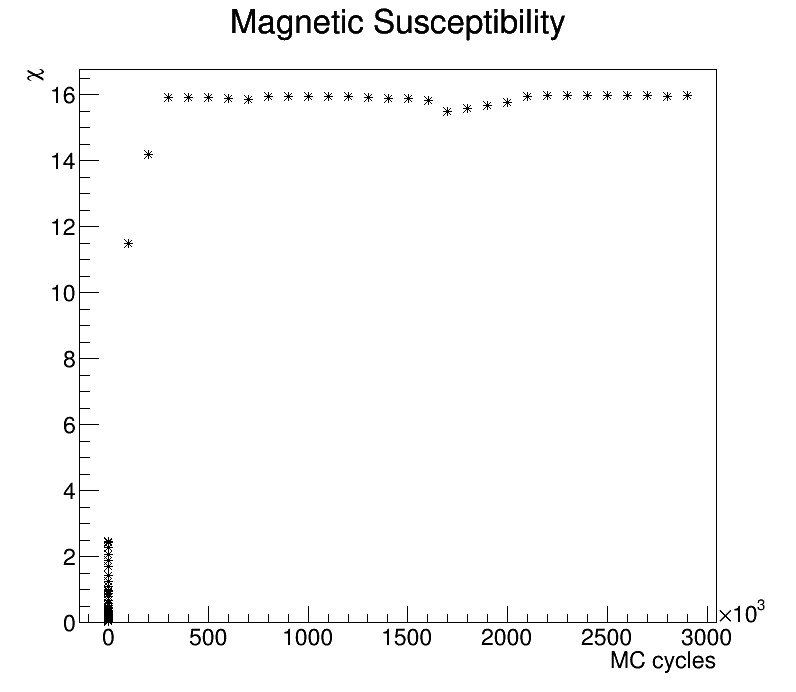
\includegraphics[width=0.3\textwidth]{benchmarks/plots/plots_random_chi_size2_temp1}
}
\caption{The (a) $<E>$, (b) $<|M|>$, (c) $C_{V}$, and (d) $\chi$ for a $2\times2$ lattice at temperature $T=1/k_{B}$.}
\label{fig:benchmarks}
\end{center}
\end{figure}

\par We also will include here a discussion of benchmarks for the random number generator itself.  In particular, all computer-algorithm random number generators are inherently deterministic.  Because a random number sequence is by definition uncorrelated, computer algorithms are incapable of producing sequences of truly random numbers. Instead, they are what are known as pseudorandom number generators.  For this reason, it is important to ensure that the random number generator being used is at least reasonably random.  Kendall and Babington Smith~\textbf{need reference} suggested a series of tests designed to check whether sequences of numbers were actually random: the frequency, serial, poker, and gap tests.  We will focus on the first three of these.\footnote{The entirety of the rest of this discussion can be found in \textbf{drueke}.}  
\par The frequency test aims to ensure that every digit occurs approximately an equal number of times in the sequence.  That is, we want to ensure that the distribution is uniform.  The frequency test for a sequence $S$ over some interval $[a,b]$ is relatively straightforward: namely, ensuring that every digit occurs in the sequence approximately 10\% of the time, as would be expected of a random sequence of digits.  However, it is important to apply the frequency test over every segment of the sequence used to ensure that there isn't a singularly bad section.  That is, we want to split the sequence into multiple blocks and ensure that, within each block, every digit still occurs about 10\% of the time.~\textbf{odell,gruenberger,drueke}
\par The serial test is designed to check that no two digits tend to occur in a particular order. This is essentially the frequency test again, but this time ensuring all groupings of two digits occur approximately 1\% of the time within the sequence.~\textbf{odell,gruenberger,drueke}
\par In the poker test, the digits in the sequence are broken into blocks of some fixed size (eg. 5 each) and then compared with might be expected in a theoretical poker hand.  In~\textbf{odell}, the only possible hands considered were pairs, three of a kind, four of a kind, and five of a kind.  We might also consider occurrences such as full houses and two pairs, as in~\textbf{babington}.  Each of these "hands" has its own likelihood of occurring.  To determine what these probabilities are, we need to determine what kind of deck we are working with.  We note already that, because we can conceivably have five of a kind in a hand, it cannot be the normal 52-card deck in four suits.  In fact, our deck is actually an infinite one, with no suits but 10 unique cards (one for each digit).  For a hand of five cards $H=(a,b,c,d,e)$, we see that each place could be any one of the 10 cards, and so there are 50 possible hands to look at.  However, to be more careful we can also look at the order in which the cards are pulled.  For example, we may have a pair $(a,a,b,c,d)$ of a pair $(a,b,c,a,d)$, and each would count as a separate hand.  So there are actually $10^{5}$ possible hands in our game of poker.  
\par How might we calculate the probability of one of the special kinds of hands of occurring?  We will now present a couple of examples.  The accepted probabilities of each of the hands is given in Table~\ref{tab:pokeracc}.  The simplest example would be five of a kind, which must always take the form $(a,a,a,a,a)$ for some $a\in\mathbb{Z}_{n}$\footnote{Here, $\mathbb{Z}_{n}=\{x\in\mathbb{Z}:0\leq x < n\}$.}.  As there are only 10 such values of $a$, there are only 10 such hands in the total of $10^{5}$ hands, and so 5 of a kind should occur with a frequency of 0.01\%.
\par Perhaps a more enlightening example is the case of four of a kind.  Here, there are 5 possible hand combinations: $(a,a,a,a,b)$, $(a,a,a,b,a)$, $(a,a,a,b,a)$, $(a,a,b,a,a)$, $(a,b,a,a,a)$, and $(b,a,a,a,a)$.  Now $a$ can represent any of the 10 digits in $\mathbb{Z}_{n}$, and $b$ can be any of those 10 digits except $a$, so there are 9 possible values of $b$ for every $a$.  As a result, we have a probability of four of a kind equal to 
$$
P(\text{4 of a kind}) = \frac{5\times10\times9}{10^{5}} = 0.45\%.
$$
Continuing in this manner (determining the number of possible hand types which will give the desired hand and multiplying by the number of possible values for each variable), we can get the results of Table~\ref{tab:pokeracc}.~\textbf{drueke}

\begin{table}[ht]
\begin{center}
\begin{tabular}{c|c} \hline
	Hand Type & Frequency (\%) \\ \hline
    5 of a Kind & 0.01\\
    4 of a Kind & 0.45\\
    3 of a Kind & 7.2\\
    2 of a Kind & 50.4\\
    Full House & 0.9\\
    Two Pair & 10.8\\ 
    Other & 30.24\\ \hline
\end{tabular}
\caption{Accepted frequencies for various poker hands~\cite{babington}.}
\label{tab:pokeracc}
\end{center}
\end{table}

\par To determine how well the output of the random number generator fits the expected values of the frequency, series, poker, and gap tests, we perform a $\chi^{2}$-test to determine the level of agreement.  This test is designed to determine whether there is any correlation between two variables $x$ and $y$.  To perform the $\chi^{2}$-test, we first compute $\chi^{2}$, which is given by
\begin{equation}
\label{eq:chi2}
\chi^{2}=\sum\frac{\left(v-v_{e}\right)^{2}}{v},
\end{equation}
where $v$ is the value observed and $v_{e}$ is the value expected~\textbf{babington}.  
\par Next, we determine the number of degrees of freedom of the problem, which is given by 
\begin{equation}
\label{eq:degfree}
DF = (n_{x}-1)*(n_{y}-1),
\end{equation}
where $n_{x}$ is the number of levels of variable $x$ and $n_{y}$ is the number of levels of variable $y$~\textbf{chi}.  It is important, therefore, to note the degrees of freedom in each of the three tests used in this analysis, as shown in Table~\ref{tab:degfree}.

\begin{table}[ht]
\begin{center}
\begin{tabular}{c|c} \hline
	Test & Degrees of Freedom \\ \hline
     Frequency Test & 9 \\
     Serial Test & 90 \\
     Poker Test & 4 \\ \hline
\end{tabular}
\caption{The degrees of freedom of the various tests used in this analysis~\textbf{babington}.}
\label{tab:degfree}
\end{center}
\end{table}

\par The final step in the $\chi^{2}$-test is to consult a $\chi^{2}$ table (or, in our case, an online $p$-value calculator~\textbf{graphpad}) to determine the $p$-value given the number of degrees of freedom and the computation of $\chi^{2}$.  This $p$-value gives the likelihood that differences in the observed and expected values is due to statistical fluctuations rather than a more fundamental error in the generation of the sequence.  In particular, we look for $p$ to be above a certain significance level, which we take to be 0.1 (although values of 0.01 and 0.05 are also common).~\textbf{drueke}
\par The five random number generators tested here are \texttt{ran0}, \texttt{ran1}, \texttt{ran2}, and \texttt{ran3} from ~\textbf{recipes}, and \texttt{rand()}, the default C++ random number generator.  \texttt{ran0} is what is known as the Minimal Standard Generator, which is a multiplicative congruential generator.  That is, it depends on the recurrence relation
\begin{equation}
\label{eq:ran0recur}
I_{j+1}=aI_{j}\mod m
\end{equation}
\texttt{ran0} specifically was proposed by Park and Miller with the settings $a=7^{5}=16807$ and $m=2^{31}-1=2147483647$.  The period of \texttt{ran0} is expected to be $2^{31}-1=2.1\times10^{9}$.~\textbf{recipes}  We found that \textt{ran0} behaves fairly well.  It passes the frequency and serial tests without much of a problem.  The only test which is does not appear to pass is the poker test.  Here, the $p$-value is $\sim0.04$, which is far below our significance threshold.  

\begin{table}[ht]
\begin{center}
\begin{tabular}{c|c|c} \hline
Statistic & Value & Significance\\\hline
$\mu$ & 4.50159 & 0.04\% \\
$\sigma$ & 2.87309 & 0.45\%\\
$\chi^{2}$ (Frequency Test) & 5.68698 & 0.7708 \\
$\chi^{2}$ (Serial Test) & 86.2657 & 0.5919 \\
$\chi^{2}$ (Poker Test) & 10.0296 & 0.0399 \\ \hline
\end{tabular}
\caption{Results of the frequency, serial, and poker tests performed on \texttt{ran0}, and the significance of those results (the percent difference from the expected value in the case of the mean $\mu$ and the standard deviation $\sigma$, and the $p$-value for the $\chi^{2}$ tests).}
\label{tab:ran0results}
\end{center}
\end{table}

\par \texttt{ran1} uses \texttt{ran0} for its random variable but also uses a shuffling algorithm developed by Bays and Durham to remove lower-order correlations.  In this shuffling, a randomly generated element of the sequence, $I_{j}$, is chosen to be output as some other element of the sequence (typically $I_{j+32}$).  According to~\textbf{recipes}, \texttt{ran1} passes all known statistical tests excepting when it is called somewhere on the order of its period ($\sim10^{8}$).~\textbf{recipes}
\par We found that this algorithm passes the frequency and poker tests, but not the serial test.  This is an interesting result as \texttt{ran1} is designed to help rid \texttt{ran0} of correlations, and \texttt{ran0} passed the serial test without a problem.  

\begin{table}[ht]
\begin{center}
\begin{tabular}{c|c|c} \hline
Statsitsic & Value & Significance\\\hline
$\mu$ & 4.50043 & 0.01\%\\
$\sigma$ & 2.87041 & 0.54\%\\
$\chi^{2}$ (Frequency Test) & 7.19849 & 0.6165\\
$\chi^{2}$ (Serial Test) & 112.818 & 0.0522\\
$\chi^{2}$ (Poker Test) & 5.22794 & 0.2647\\ \hline
\end{tabular}
\caption{Results of the frequency, serial, and poker tests performed on \texttt{ran1}, and the significance of those results (the percent difference from the expected value in the case of the mean $\mu$ and the standard deviation $\sigma$, and the $p$-value for the $\chi^{2}$ tests).}
\label{tab:ran1results}
\end{center}
\end{table}

\par Claimed to be a "perfect" random number generator (up to floating point errors) by~\textbf{recipes}, \texttt{ran2} adds another level of shuffling to further remove the correlations existing in \texttt{ran1}, as well as other randomness checks originally proposed by L'Ecuyer.  One such check is combining \texttt{ran0} and \texttt{ran1} such that the period of the sequence generated is the least common multiple of the periods of the first two algorithms.  This is done by adding the two sequences produced by these algorithms modulo the modulus $m$ of either of them.  In this way, \texttt{ran2} is designed to have a very long period ($>10^{8}$).~\textbf{recipes}
\par We found that this algorithm readily passed all of the frequency, serial, and poker tests.  In particular, it also has the lowest percent difference between the observed and expected average and standard deviation of any of the three algorithms discussed up until this point.

\begin{table}[ht]
\begin{center}
\begin{tabular}{c|c|c} \hline
Statsitsic & Value & Significance\\\hline
$\mu$ & 4.4999 & $<0.01\%$\\
$\sigma$ & 2.87382 & 0.42\%\\
$\chi^{2}$ (Frequency Test) & 8.62035 & 0.4730\\
$\chi^{2}$ (Serial Test) & 93.7899 & 0.3714\\
$\chi^{2}$ (Poker Test) & 5.28678 & 0.2591\\ \hline
\end{tabular}
\caption{Results of the frequency, serial, and poker tests performed on \texttt{ran2}, and the significance of those results (the percent difference from the expected value in the case of the mean $\mu$ and the standard deviation $\sigma$, and the $p$-value for the $\chi^{2}$ tests).}
\label{tab:ran2results}
\end{center}
\end{table}

\par \texttt{ran3} was originally presented by Knuth and is in fact based on subtractive methods rather than acting as a linear congruential method.  These subtractive methods make \texttt{ran3} a Fibonacci generator.  The idea here is that the next term in the sequence comes from the subtraction of two previous terms.  In particular,
\begin{equation}
\label{eq:fibgen}
x_{k}=x_{k-a}-x_{k-b}
\end{equation}
for some fixed $a,b\in\mathbb{Z}$ known as lags.  Fibonacci generators are typically very efficient and pass most randomness tests thrown at them, although they do require more storage than linear congruential algorithms.~\textbf{fib}
\par We found that, indeed, \texttt{ran3} passed all three of the frequency, serial, and poker tests, just as did \texttt{ran2}.  However, this algorithm had much lower $p$-values for the serial and poker tests than did \texttt{ran2}, indicating that perhaps this is not the stronger of the two.

\begin{table}[ht]
\begin{center}
\begin{tabular}{c|c|c} \hline
Statsitsic & Value & Significance\\\hline
$\mu$ & 4.50161 & 0.04\%\\
$\sigma$ & 2.87307 & 0.45\%\\
$\chi^{2}$ (Frequency Test) & 5.92085 & 0.7478\\
$\chi^{2}$ (Serial Test) & 106.29 & 0.1157\\
$\chi^{2}$ (Poker Test) & 7.28835 & 0.1214\\ \hline
\end{tabular}
\caption{Results of the frequency, serial, and poker tests performed on \texttt{ran3}, and the significance of those results (the percent difference from the expected value in the case of the mean $\mu$ and the standard deviation $\sigma$, and the $p$-value for the $\chi^{2}$ tests).}
\label{tab:ran3results}
\end{center}
\end{table}

\par The final random number generator tested in this analysis is the standard \texttt{rand()} function in the standard C++ library.  According to the C++ documentation, the default underlying algorithm here is another linear congruential algorithm.  We chose to test this algorithm primarily as a check that the code created to run the four randomness tests was working properly, working under the assumption that, as it comes standard, it has likely been well-tested at this point.
\par We found that, as expected, \texttt{ran4} passed the frequency, serial, and poker tests with flying colors.  However, it failed the gap test (as did the other four random number generators tested).  This result leads the author to believe that the code used in the gap test is flawed somehow, and that further study is needed before any claims can be made.

\begin{table}[ht]
\begin{center}
\begin{tabular}{c|c|c} \hline
Statistic & Value & Significance\\\hline
$\mu$ & 4.50236 & 0.05\%\\
$\sigma$ & 2.87138 & 0.51\%\\
$\chi^{2}$ (Frequency Test) & 7.25112 & 0.6110 \\
$\chi^{2}$ (Serial Test) & 79.4787 & 0.7784 \\
$\chi^{2}$ (Poker Test) & 3.55947 & 0.4689 \\ \hline
\end{tabular}
\caption{Results of the frequency, serial, poker, and gap tests performed on \texttt{ran4}, and the significance of those results (the percent difference from the expected value in the case of the mean $\mu$ and the standard deviation $\sigma$, and the $p$-value for the $\chi^{2}$ tests).}
\label{tab:ran4results}
\end{center}
\end{table}

\section{Results}
\label{sec:results}

To test our algorithm, we looked first at a $20\times20$ lattice to determine how many MC cycles would be needed to reach the steady state.  Looking first at a temperature of $T=1/k_{B}$, we plotted $<E>$, $<|M|>$, $C_{V}$, and $\chi$ against the number of cycles used in the computation.  The results are in Fig.~\ref{fig:size20temp1rando} for a random initial state and in Fig.~\ref{fig:size20temp1steady} for a steady initial state. 

\begin{figure}[h]
\begin{center}
\subfigure[]{
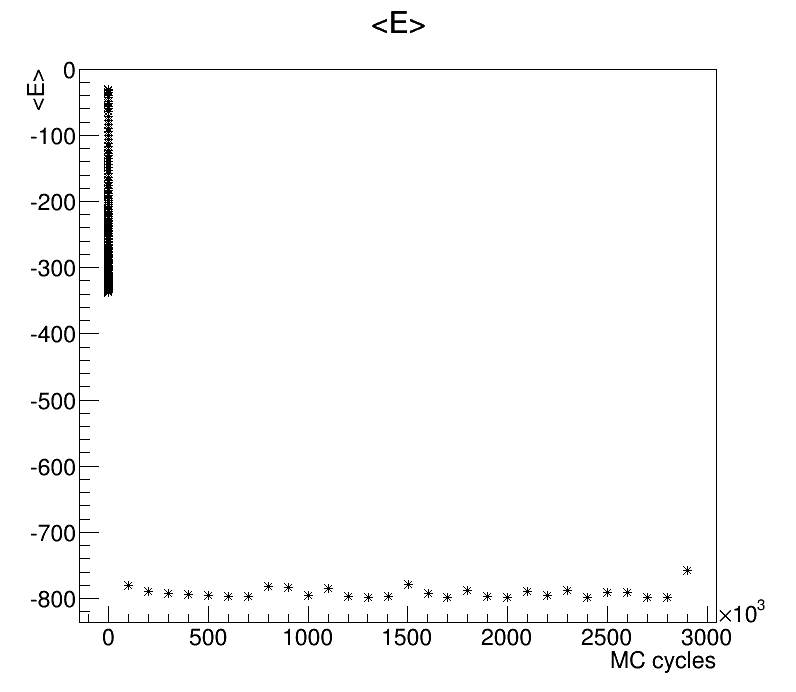
\includegraphics[width=0.3\textwidth]{plots/partcandd/plots_random_meanE_size20_temp1}
}
\subfigure[]{
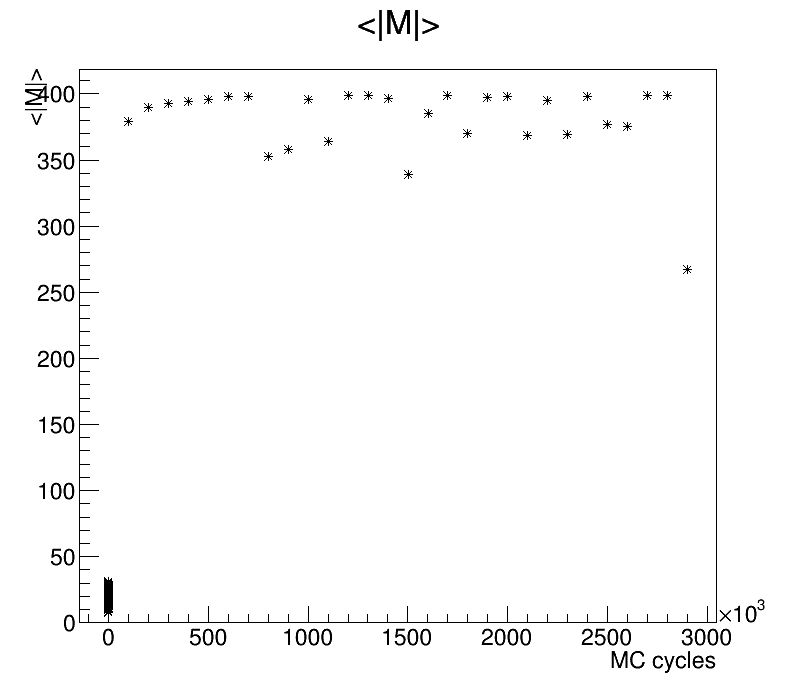
\includegraphics[width=0.3\textwidth]{plots/partcandd/plots_random_meanAbsM_size20_temp1}
} \\
\subfigure[]{
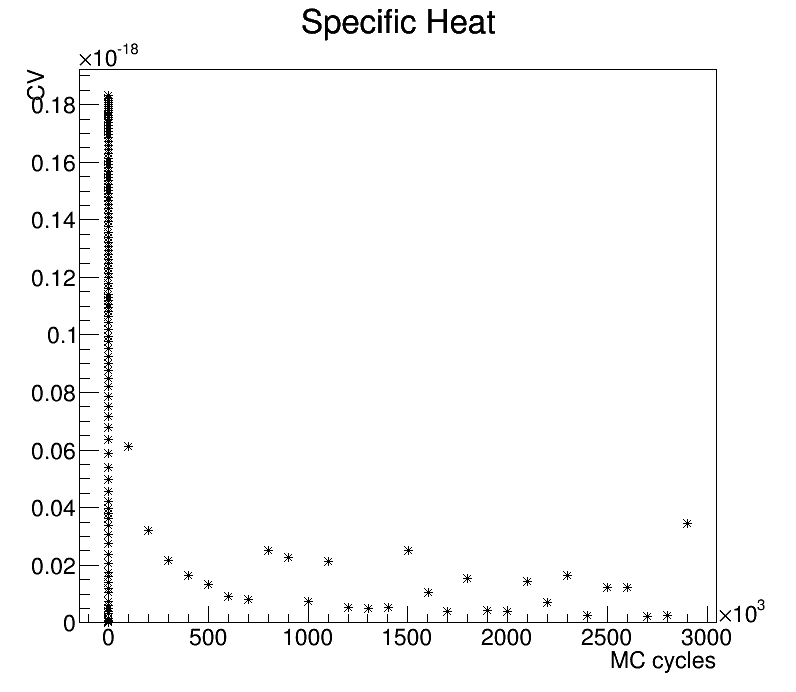
\includegraphics[width=0.3\textwidth]{plots/partcandd/plots_random_CV_size20_temp1}
}
\subfigure[]{
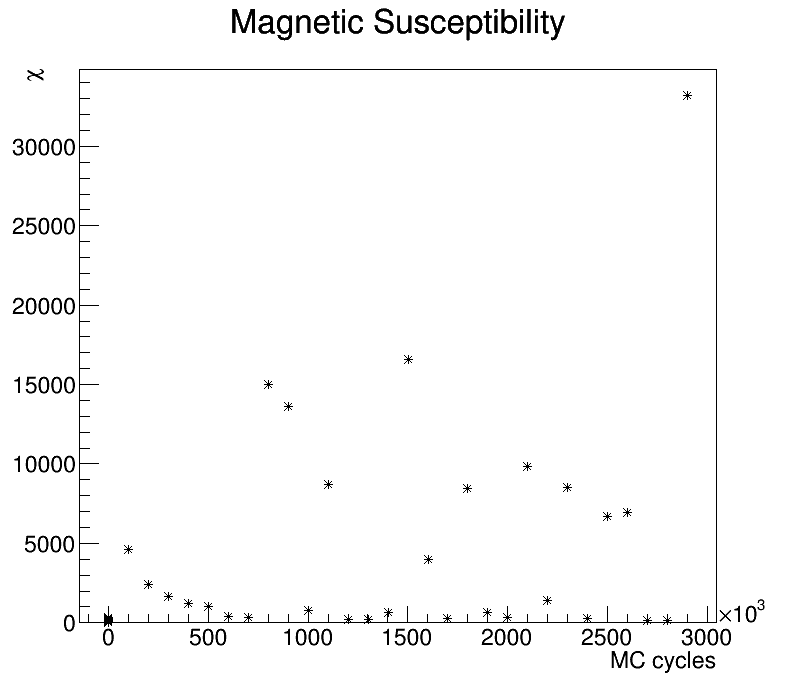
\includegraphics[width=0.3\textwidth]{plots/partcandd/plots_random_chi_size20_temp1}
}
\caption{Statistical quantities for a $20\times20$ lattice at a temperature $T=1/k_{B}$ with an initial state of a random selection of spins.}
\label{fig:size20temp1rando}
\end{center}
\end{figure}

\par We see that we are able to get good results for $<E>$ and $<|M|>$ after very few MC cycles in both the initial random and the initial steady states, although there was a much wider variation in the values produced for these quantities when the initial state was random.  This is not suprising given that the steady state starts right near the accepted value for these quantities and only varies with a small probability from that central value, whereas the initial random state needs to find the accepted value from some random initial state.  We also see much less variation once the steady state is reached for the initial steady state.  Generally, though, the number of MC cycles required to reach the equilibrium values didn't seem to depend much on the initial state of the lattice for such a small lattice size, although starting in the steady state was a bit faster.  

\begin{figure}[h]
\begin{center}
\subfigure[]{
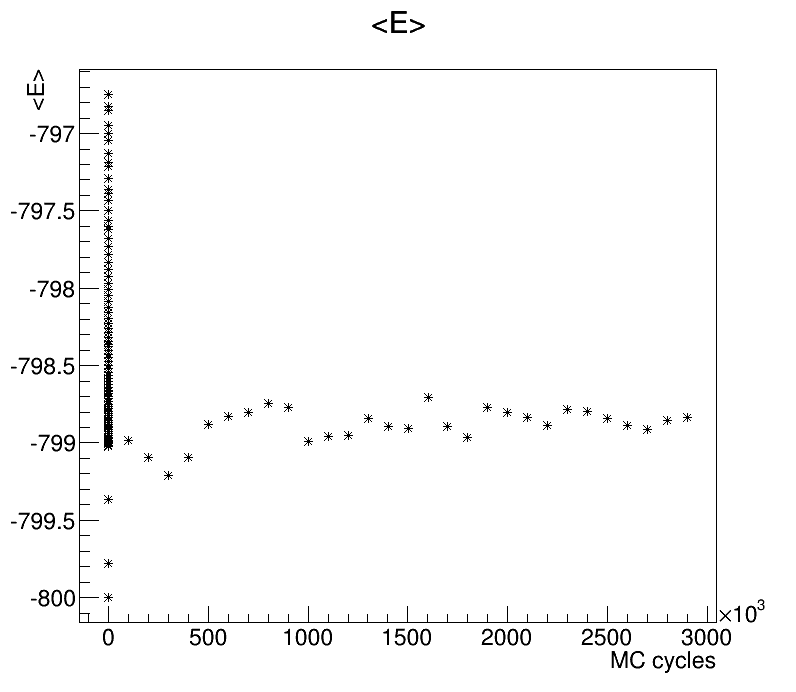
\includegraphics[width=0.3\textwidth]{plots/partcandd/plots_steady_meanE_size20_temp1}
}
\subfigure[]{
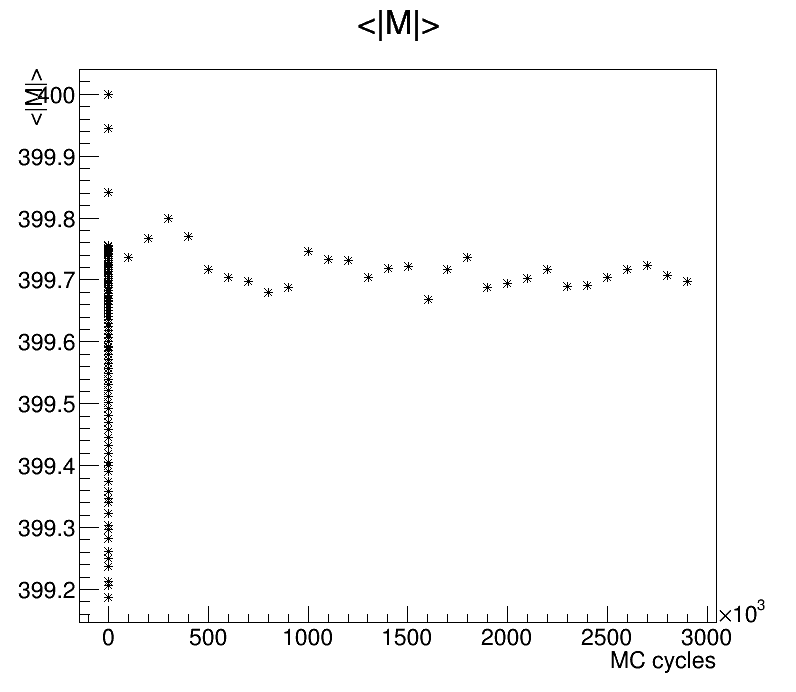
\includegraphics[width=0.3\textwidth]{plots/partcandd/plots_steady_meanAbsM_size20_temp1}
} \\
\subfigure[]{
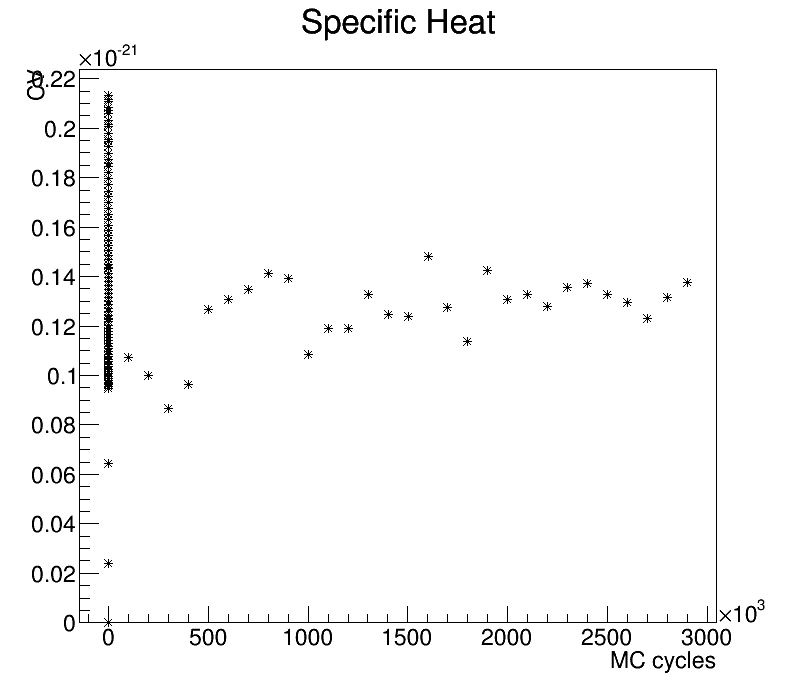
\includegraphics[width=0.3\textwidth]{plots/partcandd/plots_steady_CV_size20_temp1}
}
\subfigure[]{
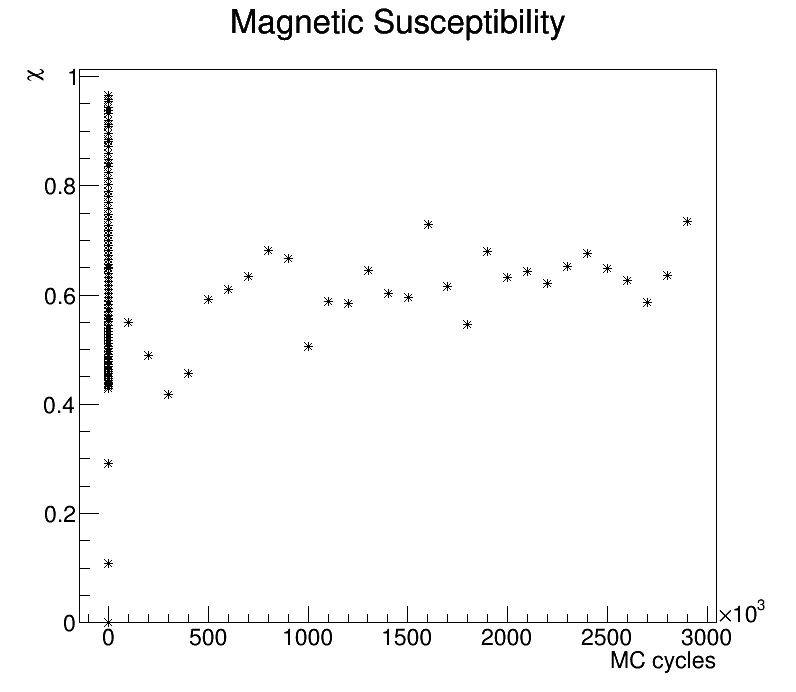
\includegraphics[width=0.3\textwidth]{plots/partcandd/plots_steady_chi_size20_temp1}
}
\caption{Statistical quantities for a $20\times20$ lattice at a temperature $T=1/k_{B}$ with a steady-state initial state.}
\label{fig:size20temp1steady}
\end{center}
\end{figure}

\par We also wanted to look at how the number of MC cycles required to reach the steady state approximation might depend on temperature.  Thus, we repeated the analysis of our expectation values, $C_{V}$, and $\chi$ using $T=2.4/k_{B}$.  The results are shown in Fig.~\ref{fig:size20temp24rando} for the random initial state and Fig.~\ref{fig:size20temp24steady} for the initial steady state. Here, we see that there is a distinct difference between the number of MC cycles required to reach the equilibrium values for the statistical quantities, which is particularly noticeable in the $C_{V}$ plots.  We see that with the random initial state, we require $\sim500\times10^{3}$ MC cycles to reach the equilibrium value for $C_{V}$, but only $\sim400\times10^{3}$ or less for the initial steady state.  Both of these values, though are much larger than the number of cycles required with $T=1/k_{B}$, which is $\sim100\times10^{3}$ for the initial steady state and $\sim 300\times10^{3}$ for the random initial state.  

\begin{figure}[h]
\begin{center}
\subfigure[]{
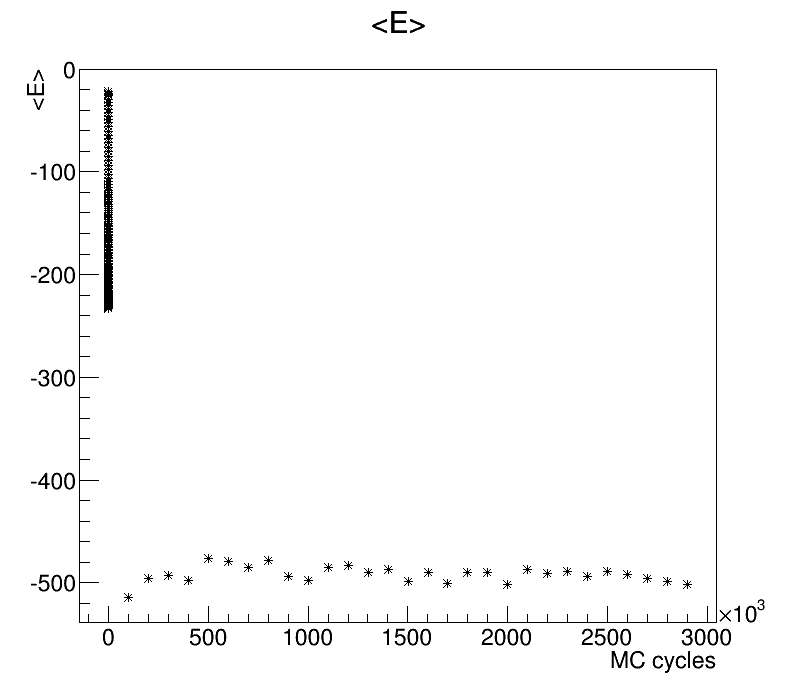
\includegraphics[width=0.3\textwidth]{plots/partcandd/plots_random_meanE_size20_temp24}
}
\subfigure[]{
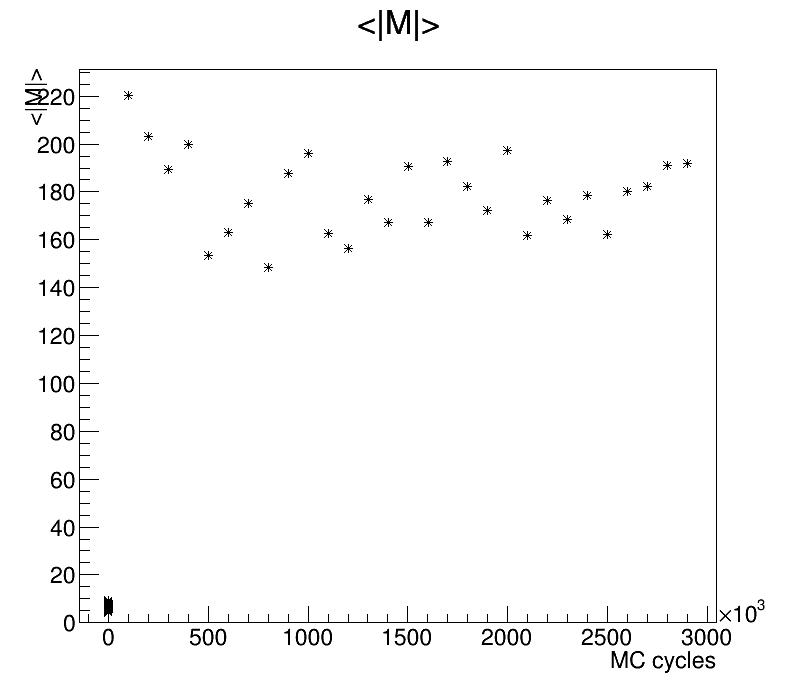
\includegraphics[width=0.3\textwidth]{plots/partcandd/plots_random_meanAbsM_size20_temp24}
} \\
\subfigure[]{
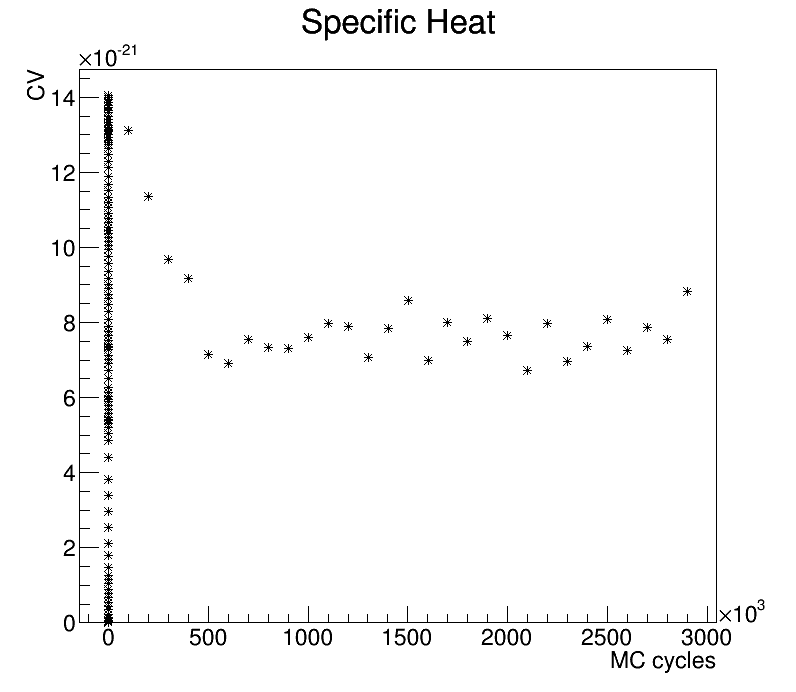
\includegraphics[width=0.3\textwidth]{plots/partcandd/plots_random_CV_size20_temp24}
}
\subfigure[]{
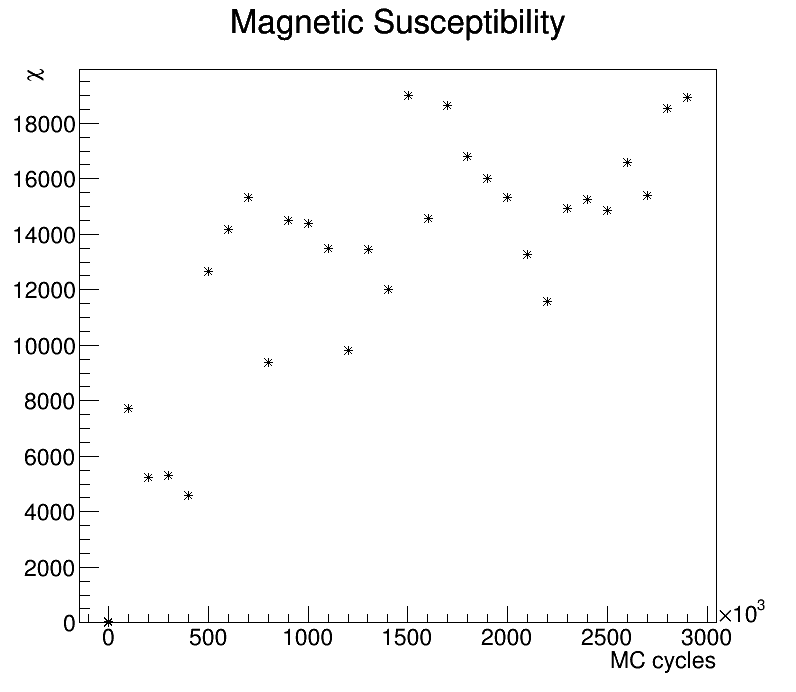
\includegraphics[width=0.3\textwidth]{plots/partcandd/plots_random_chi_size20_temp24}
}
\caption{Statistical quantities for a $20\times20$ lattice at a temperature $T=2.4/k_{B}$ with an initial state of a random selection of spins.}
\label{fig:size20temp24rando}
\end{center}
\end{figure}
 
\par One interesting feature of Fig.~\ref{fig:size20temp24rando} and Fig.~\ref{fig:size20temp24steady} is that the magnetic susceptibility never seems to reach a reasonable equilibrium value, regardless of the number of MC cycles.  Even in Fig.~\ref{fig:size20temp1rando} and Fig.~\ref{fig:size20temp1steady}, $\chi$ has a large variation and doesn't approach the equililbrium value strongly.  It may be possible that this is due to the fact that $<M>$, rather than $<|M|>$, was used in the calculation.

\begin{figure}[h]
\begin{center}
\subfigure[]{
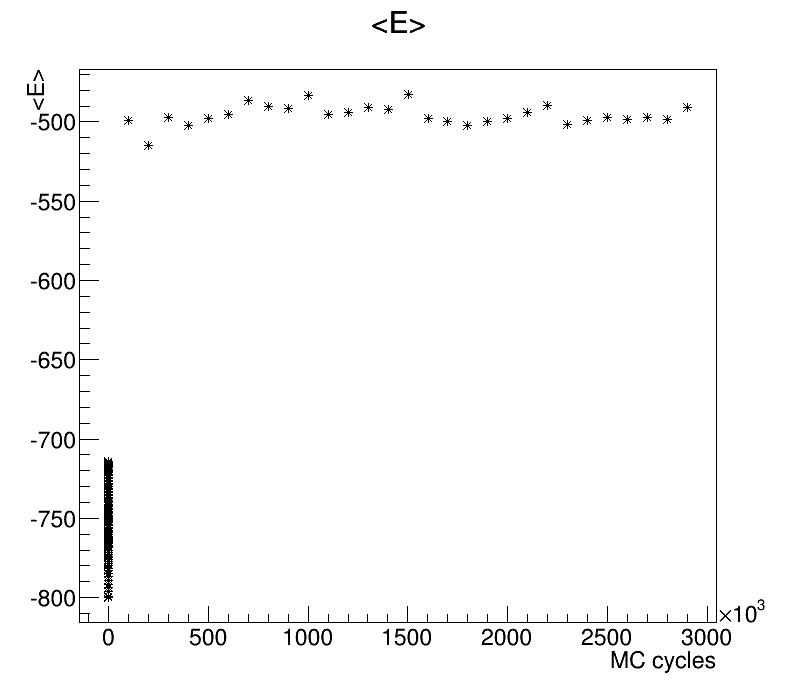
\includegraphics[width=0.3\textwidth]{plots/partcandd/plots_steady_meanE_size20_temp24}
}
\subfigure[]{
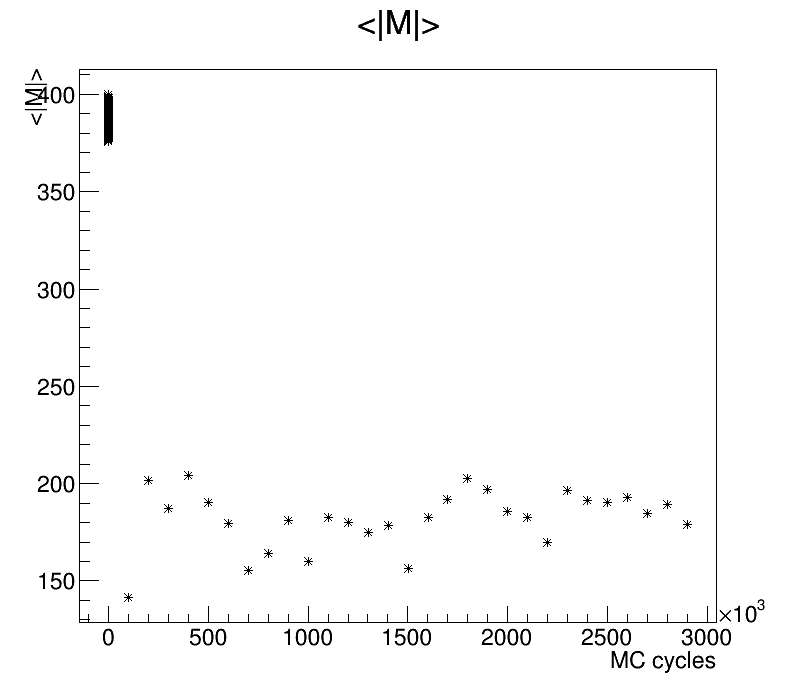
\includegraphics[width=0.3\textwidth]{plots/partcandd/plots_steady_meanAbsM_size20_temp24}
} \\
\subfigure[]{
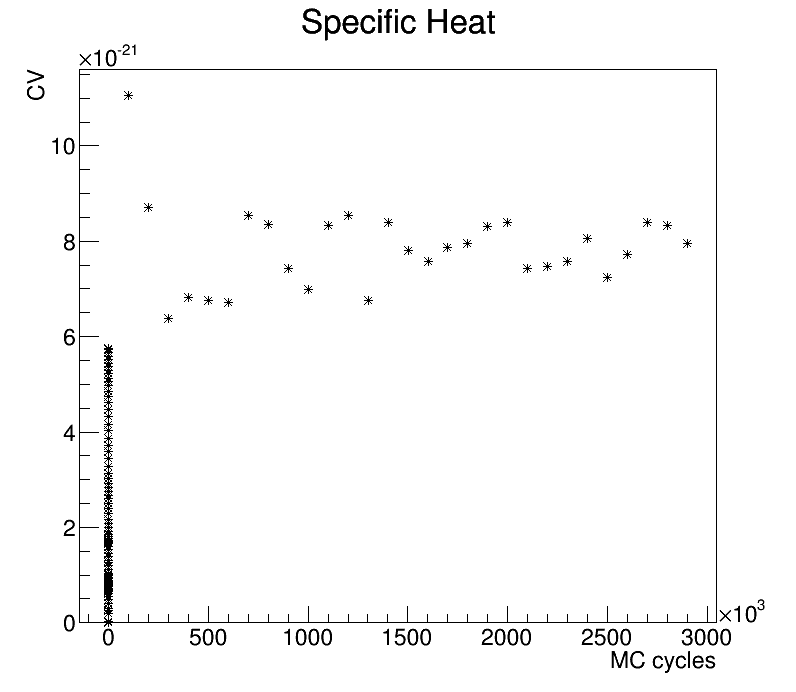
\includegraphics[width=0.3\textwidth]{plots/partcandd/plots_steady_CV_size20_temp24}
}
\subfigure[]{
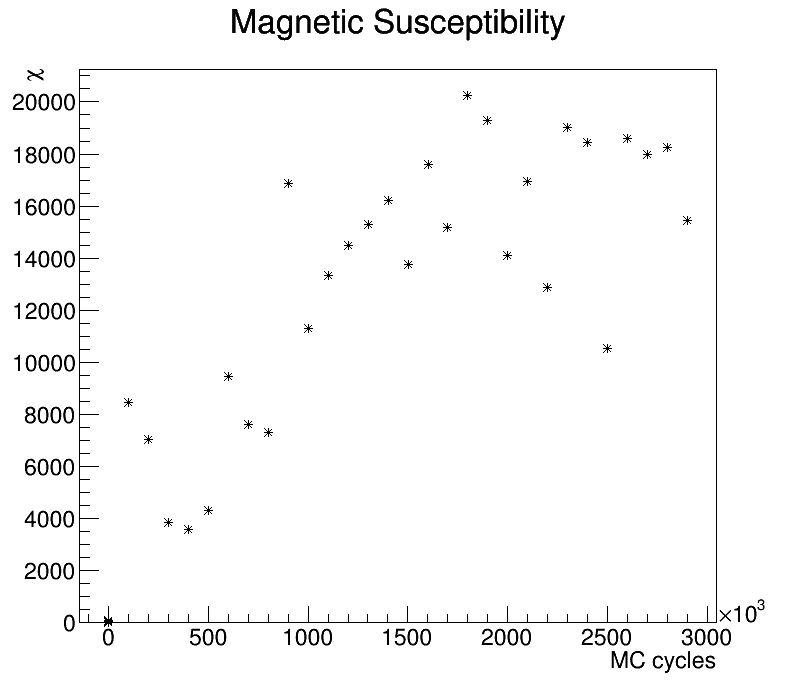
\includegraphics[width=0.3\textwidth]{plots/partcandd/plots_steady_chi_size20_temp24}
}
\caption{Statistical quantities for a $20\times20$ lattice at a temperature $T=2.4/k_{B}$ with a steady-state initial state.}
\label{fig:size20temp24steady}
\end{center}
\end{figure}

\par We next looked at the probability of various energies in the calculation, $P(E)$, defined to be the number of times a given energy $E$ occurs in the MC process divided by the number of cycles used.  The results starting from the steady state are shown in Fig.~\ref{fig:size20pofE}.  As we can see, at both temperatures, the most likely energy is the equlibrium energy.  However, there are far fewer energies used in the calculation for the lower-temperature system.  It is reasonable to look to the $C_{V}$ plots in Fig.~\ref{fig:size20temp1steady} and Fig.~\ref{fig:size20temp24steady}, because $C_{V}$ is the variance of $E$ up to a multiplicative factor.  We see that $C_{V}\approx0.12$ for $T=1/k_{B}$ but $C_{V}\approx8$ for $T=2.4/k_{B}$.  This implies that we would expect a far larger variation in possible energy values for the higher temperature system.

\begin{figure}[h]
\begin{center}
\subfigure[]{
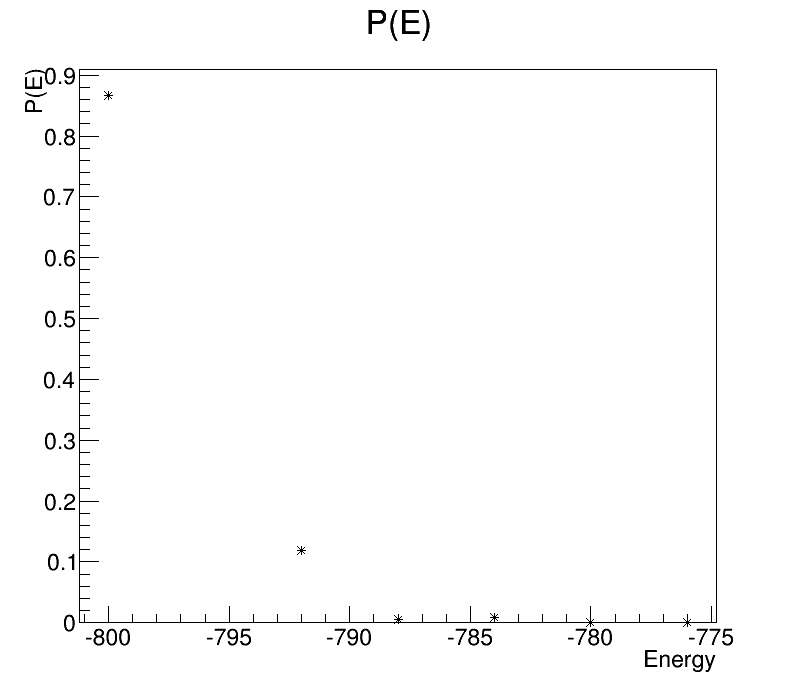
\includegraphics[width=0.3\textwidth]{plots/partcandd/plots_steady_pofE_size20_temp1}
}
\subfigure[]{
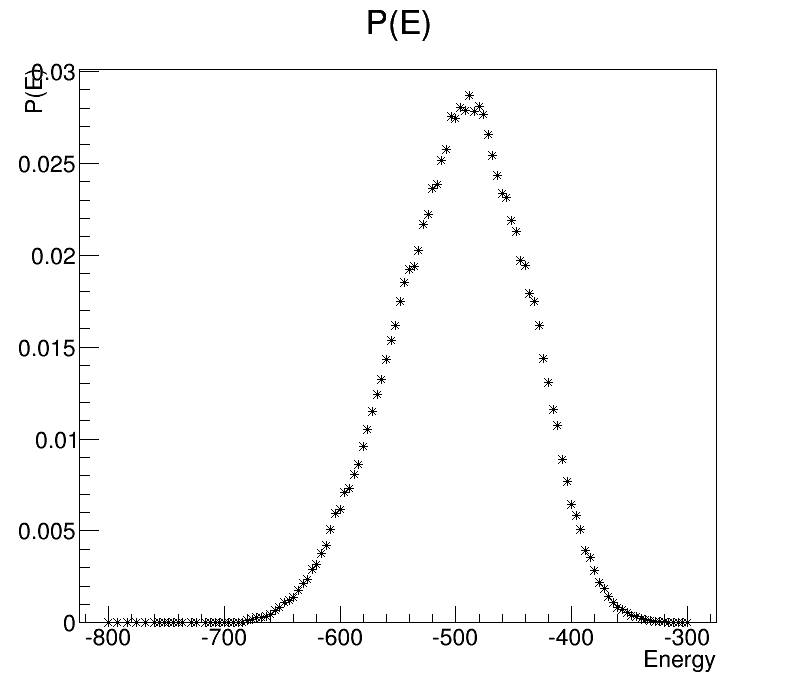
\includegraphics[width=0.3\textwidth]{plots/partcandd/plots_steady_pofE_size20_temp24}
} 
\caption{$P(E)$ for a $20\times20$ lattice at a temperature of (a) $T=1/k_{B}$ and (b) $T=2.4/k_{B}$.}
\label{fig:size20pofE}
\end{center}
\end{figure}

\par This is all well and good, but we would like now to do some physics with our Ising model calculation.  In particular, we can look at phase transitions by investigating the various statistical mechanical properties which we been focusing on.  A phase transition is when the matter undergoes a change of phase (eg. liquid to gas or solid to liquid, etc.).  It occurs at the critical temperature of the system, denoted $T_{C}$.  Near $T_{C}$, many physical quantities can be characterized by a power law exponent.  For example, the mean magnetization is given by
\begin{equation}
\label{eq:tcmag}
<M(T)>\sim(T-T_{C})^{1/8},
\end{equation}
the heat capacity by
\begin{equation}
\label{eq:tccv}
C_{V}(T)\sim|T_{C}-T|^{0},
\end{equation}
and the susceptibility by
\begin{equation}
\label{eq:tcchi}
\chi(T)\sim|T-T_{C}|^{\frac{7}{4}}.
\end{equation}
In addition, with the introduction of $T_{C}$, we can introduce the correlation length $\xi$, which is a measure of how correlated the spins within the lattice are to one another.  It is expected that $\xi$ is on the order of the lattice spacing for $T>>T_{C}$, but increases drastically as
\begin{equation}
\label{eq:tccorr}
\xi(T)\sim|T_{C}-T|^{-\nu}
\end{equation}
for $T$ near $T_{C}$ because near $T_{C}$ the spins begin to correlate more and more~\textbf{lecture notes}.
\par At a second-order phase transition, we expect $\xi$ to span the whole system.  This becomes a problem because we are restricted to finite-sized lattices.  However, this means that $\xi$ will scale with the size of the lattice, and so we can use a finite lattice to approximate an infinite system.  In particular, the critical temperature will scale as
\begin{equation}
\label{eq:tcscale}
T_{C}(L=n)-T_{C}(L=\infty)=an^{\frac{1}{\nu}}
\end{equation}
for some constant $a$ for a lattice of size $L=n$.  By setting $T=T_{C}$, we can then see that~\eqref{eq:tcmag},~\eqref{eq:tccv}, and~\eqref{eq:tcchi} become~\textbf{lecture notes}
\begin{align}
\label{eq:tcquants}
<M(T)> & \sim  (T-T_{C})^{\frac{1}{8}} \rightarrow  L^{\frac{1}{8\nu}} \\
C_{V}(T) & \sim  |T_{C}-T|^{-\frac{7}{4}} \rightarrow  L^{0} \\
\chi(T) & \sim  |T_{C}-T|^{0} \rightarrow L^{\frac{7}{4\nu}}. 
\end{align}
\par In order to study $T_{C}$, we look for indications of a phase transition in the graphs of $<E>$, $<|M|>$, $C_{V}$, and $\chi$\footnote{Here, $\chi$ is calculated with $<|M|>$.} for various lattice sizes.  These plots are shown in Fig.~\ref{fig:latsize20}, Fig.~\ref{fig:latsize40}, Fig~\ref{fig:latsize60}, and Fig.~\ref{fig:latsize80}.  They are made with $10^{6}$ MC cycles at each temperature.

\begin{figure}[h]
\begin{center}
\subfigure[]{
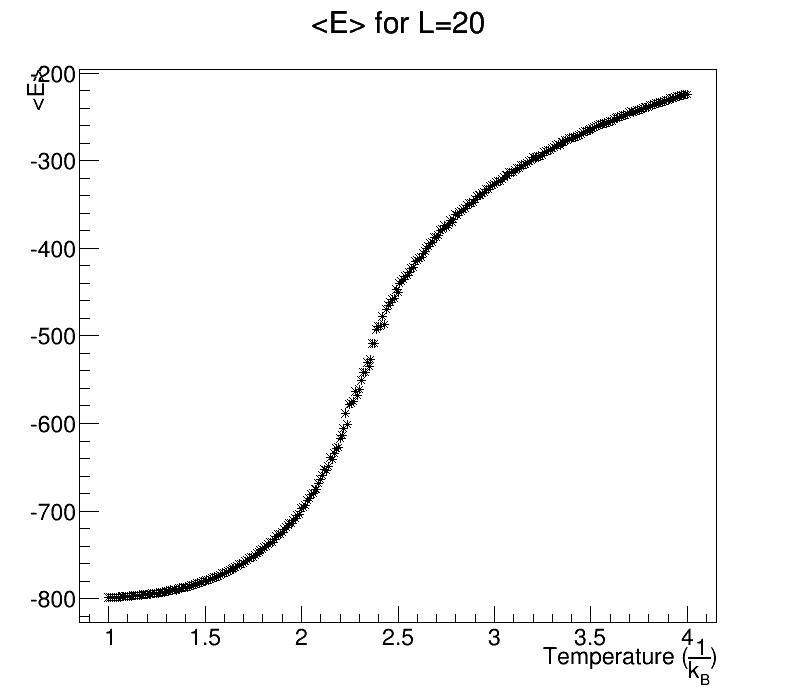
\includegraphics[width=0.3\textwidth]{plots/parte/expE_latsize20}
}
\subfigure[]{
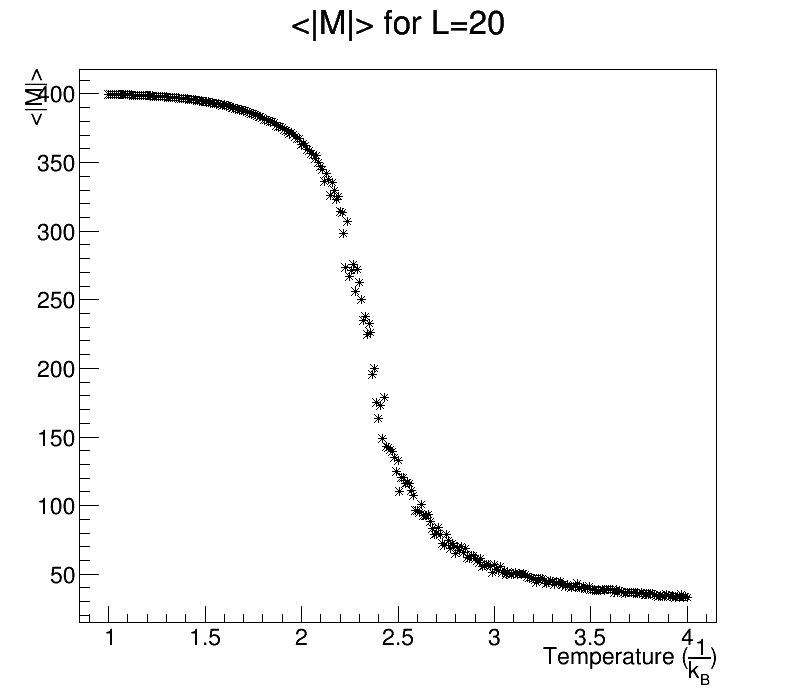
\includegraphics[width=0.3\textwidth]{plots/parte/expAbsM_latsize20}
} \\
\subfigure[]{
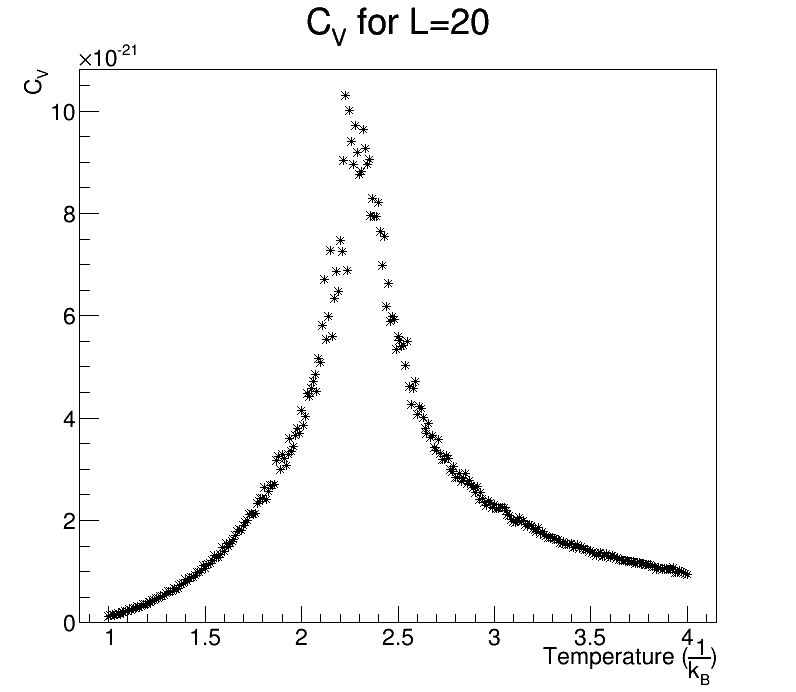
\includegraphics[width=0.3\textwidth]{plots/parte/CV_latsize20}
}
\subfigure[]{
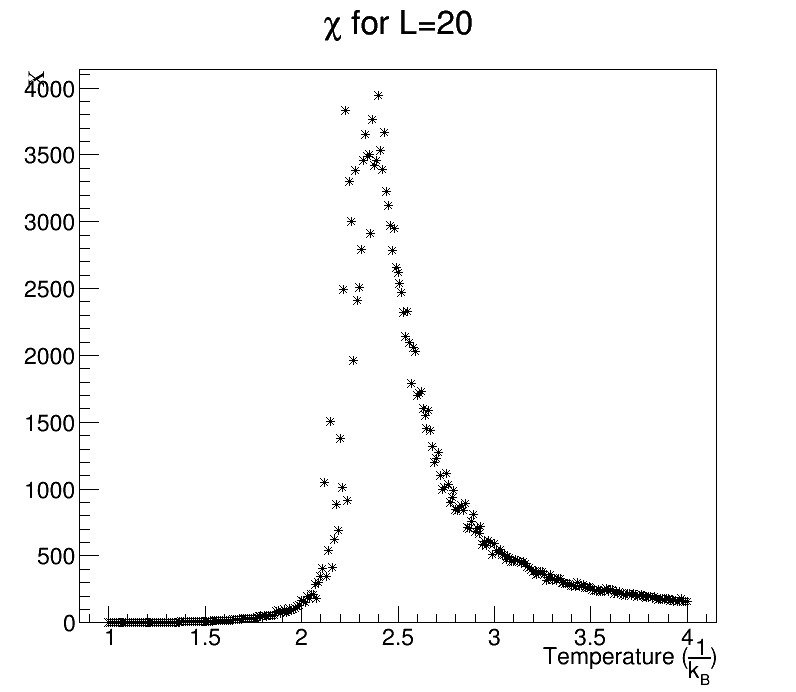
\includegraphics[width=0.3\textwidth]{plots/parte/susceptibility_latsize20}
}
\caption{Statistical quantities for a $20\times20$ lattice with a steady initial state plotted against the temperature.}
\label{fig:latsize20}
\end{center}
\end{figure}

\par In all of the plots, the evidence of a phase transition is obvious.  Just before $T=2.5/k_{B}$, the $<E>$ curve slopes sharply upward, the $<|M|>$ curve slopes sharply downward, and both $C_{V}$ and $\chi$ peak sharply.  In particular, we can note that the peak is sharper to the left in these cases, and has a somewhat longer tail.

\begin{figure}[h]
\begin{center}
\subfigure[]{
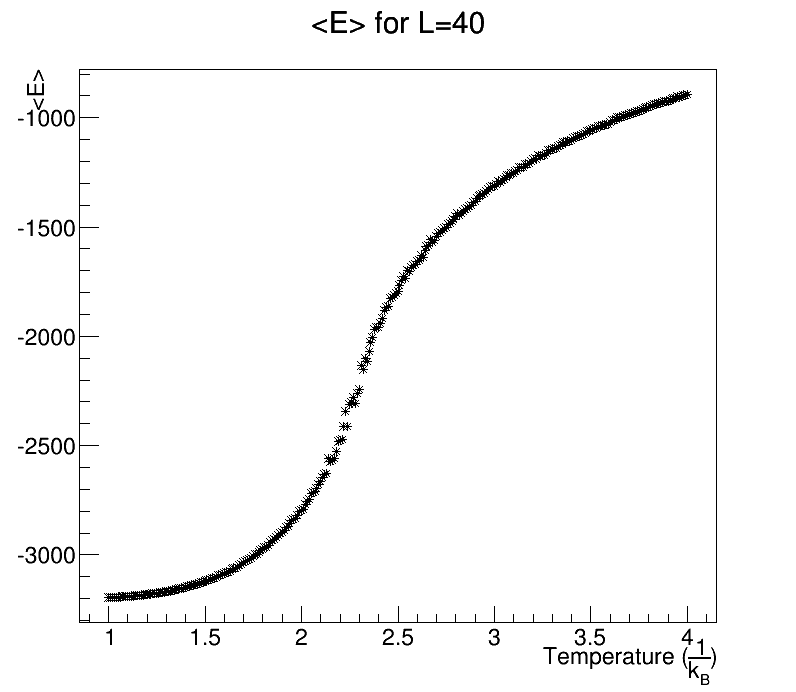
\includegraphics[width=0.3\textwidth]{plots/parte/expE_latsize40}
}
\subfigure[]{
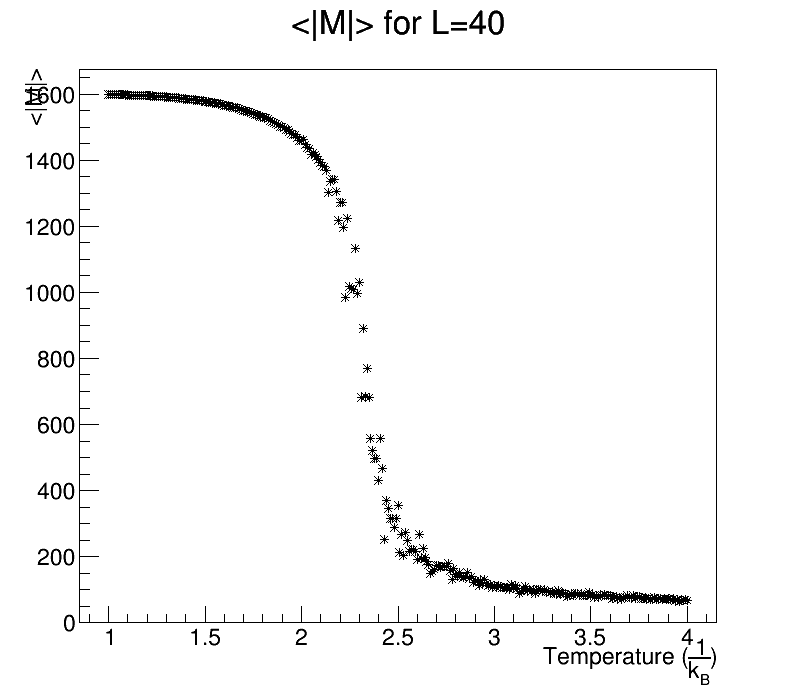
\includegraphics[width=0.3\textwidth]{plots/parte/expAbsM_latsize40}
} \\
\subfigure[]{
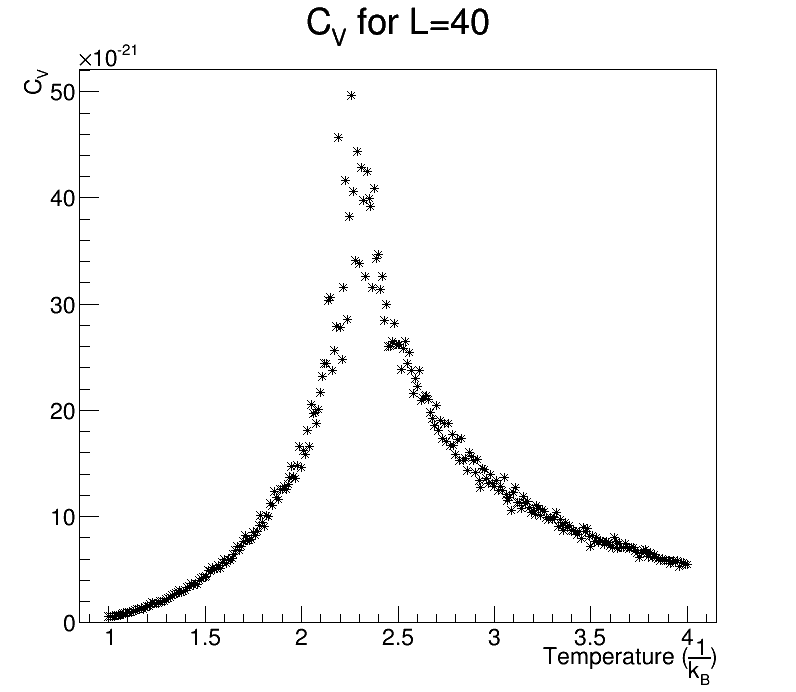
\includegraphics[width=0.3\textwidth]{plots/parte/CV_latsize40}
}
\subfigure[]{
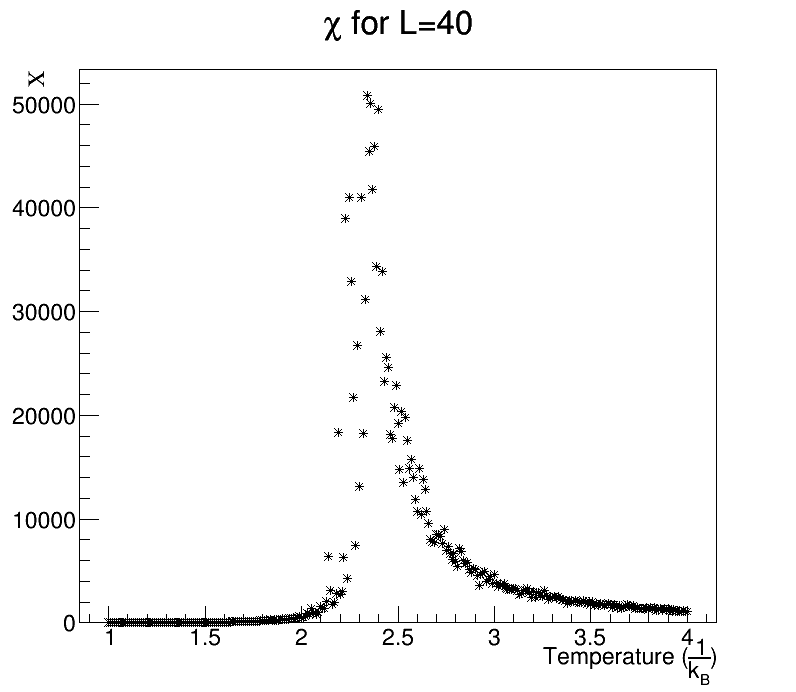
\includegraphics[width=0.3\textwidth]{plots/parte/susceptibility_latsize40}
}
\caption{Statistical quantities for a $40\times40$ lattice with a steady initial state plotted against the temperature.}
\label{fig:latsize40}
\end{center}
\end{figure}

\par We wish to use these results to determine $T_{C}$ in the limit $L\rightarrow\infty$, using $\nu=1$.  The accepted value is given by $T_{C}=2.269/k_{B}$~\textbf{lecture}.    We can use~\eqref{eq:tcscale} to calculate $T_{C}(L=\infty)$ from our plots.  To do this, we need the information of $T_{C}(L)$.  This is found in Table~\ref{tab:tcl}. 

\begin{table}[ht]
\begin{center}
\begin{tabular}{c|c|c|c} \hline
L & $T_{C}$ ($1/k_{B}$) (from $C_{V}$) & $T_{C}$ ($1/k_{B}$) (from $\chi$) & Average $T_{C}$ ($1/k_{B}$)\\ \hline
20 & 2.25 & 2.35 & 2.30 \\
40 & 2.30 & 2.35 & 2.33 \\
60 & 2.35 & 2.40 & 2.38 \\
80 & 2.40 & 2.45 & 2.43\\ \hline
\end{tabular}
\caption{Approximate values for $T_{C}(L)$ for $L=20, 40, 60,$ and 80 used with~\eqref{eq:tcscale} to determine $T_{C}(L=\infty)$.}
\label{tab:tcl}
\end{center}
\end{table}

\par  Now we know 
$$
T_{C}(L=\infty)=T_{C}(L)-aL^{-1},
$$
for some $a\in\mathbb{R}$.  So
\begin{align*}
T_{C}(L=\infty) & = \frac{2.30}{k_{B}}-\frac{a}{20} \\
T_{C}(L=\infty) & = \frac{2.33}{k_{B}}-\frac{a}{40} \\
T_{C}(L=\infty) & = \frac{2.38}{k_{B}}-\frac{a}{60} \\
T_{C}(L=\infty) & = \frac{2.43}{k_{B}}-\frac{a}{80}.
\end{align*}
\par Because~\eqref{eq:tcscale} gives us to equations in 2 unknowns, and there we are looking at four different lattice sizes, we can get any number of 8 possible solutions for $T_{C}$ and $a$.  After performing these calculations in Mathematica~\textbf{need reference}, we see get the possible solutions shown in Fig.~\ref{fig:tcsolve}.  That is, we have $\frac{2.35}{k_{B}}\leq T_{C}\leq\frac{2.575}{k_{B}}$.  This is an error of anywhere between $3.57\%\leq\sigma\leq13.49\%$ compared with the accepted result of $2.269/k_{B}$~\textbf{lectures}.  Given that our values for $T_{C}(L)$ were estimated by eye from the graphs, this is a very reasonable result.

\begin{figure}[h]
\begin{center}
\subfigure[]{
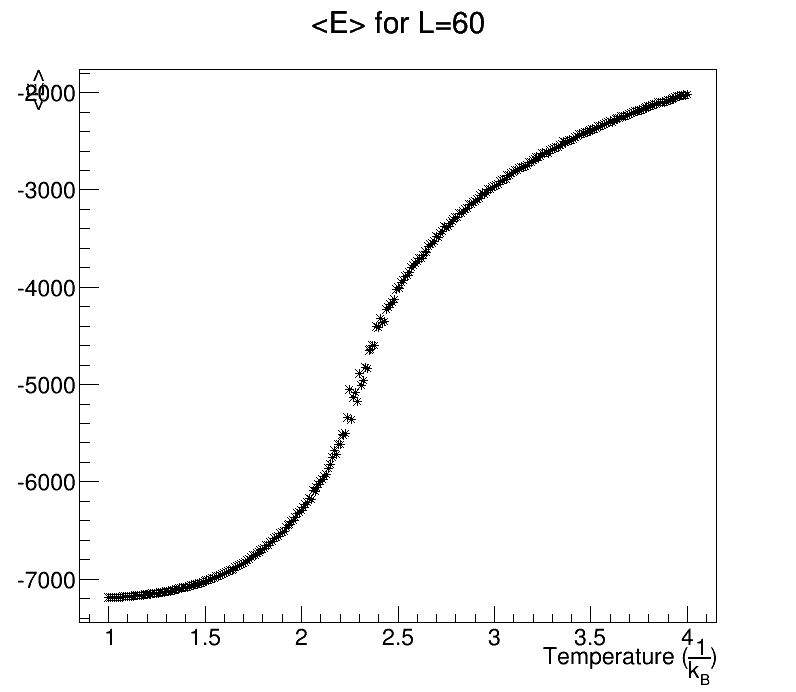
\includegraphics[width=0.3\textwidth]{plots/parte/expE_latsize60}
}
\subfigure[]{
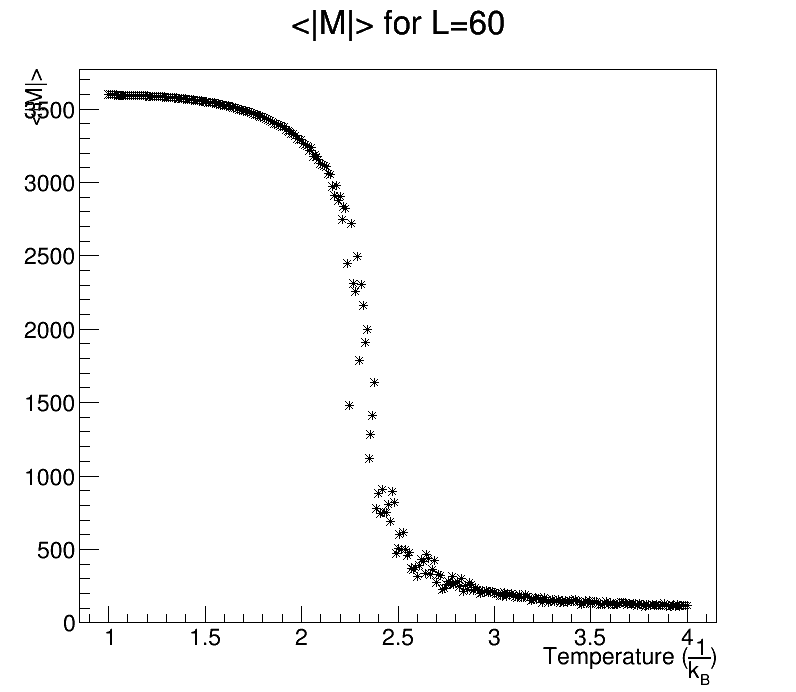
\includegraphics[width=0.3\textwidth]{plots/parte/expAbsM_latsize60}
} \\
\subfigure[]{
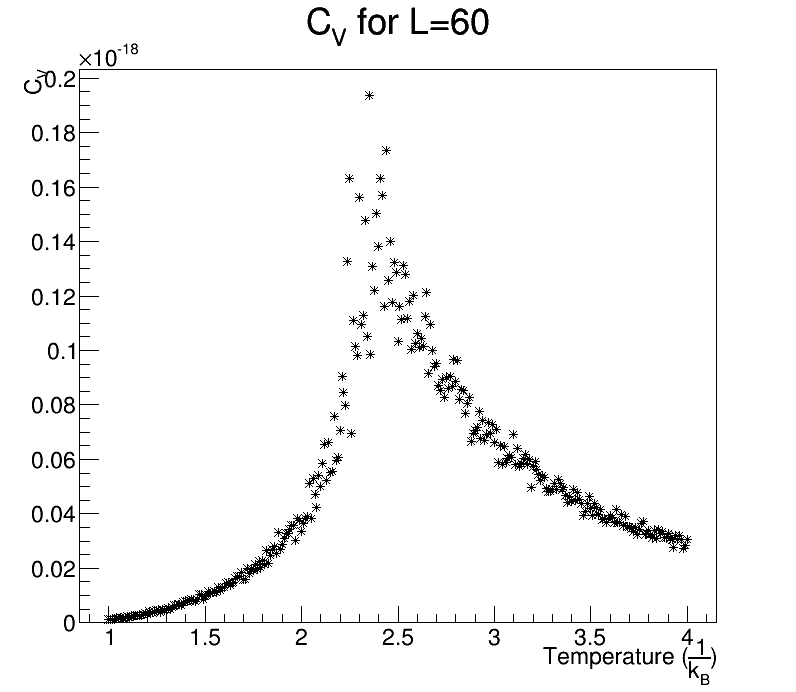
\includegraphics[width=0.3\textwidth]{plots/parte/CV_latsize60}
}
\subfigure[]{
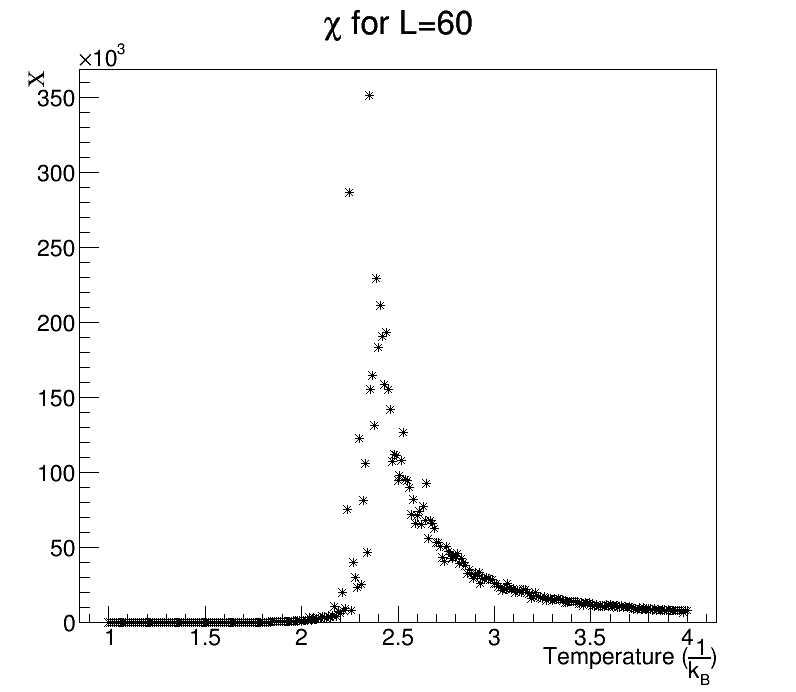
\includegraphics[width=0.3\textwidth]{plots/parte/susceptibility_latsize60}
}
\caption{Statistical quantities for a $60\times60$ lattice with a steady initial state plotted against the temperature.}
\label{fig:latsize60}
\end{center}
\end{figure}

\begin{figure}[h]
\begin{center}
\subfigure[]{
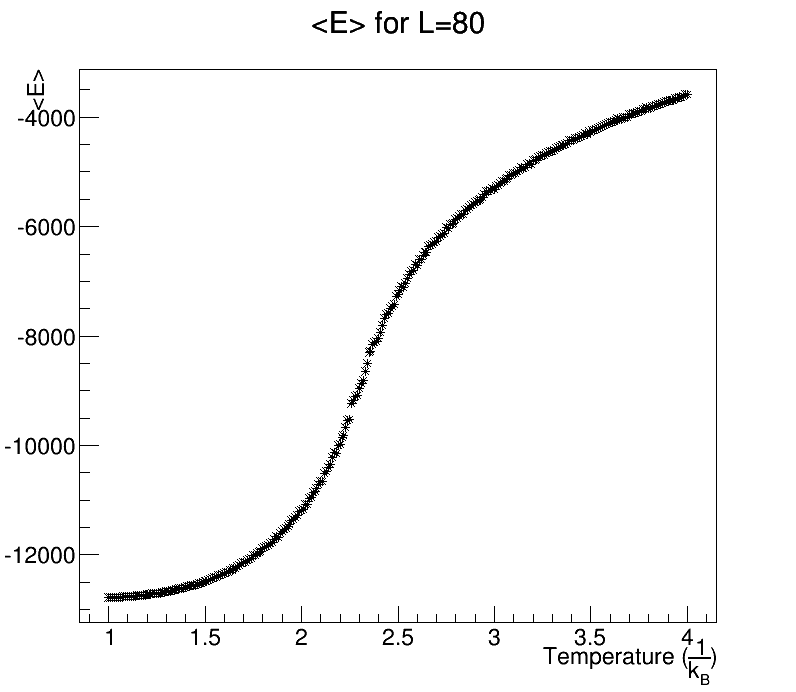
\includegraphics[width=0.3\textwidth]{plots/parte/expE_latsize80}
}
\subfigure[]{
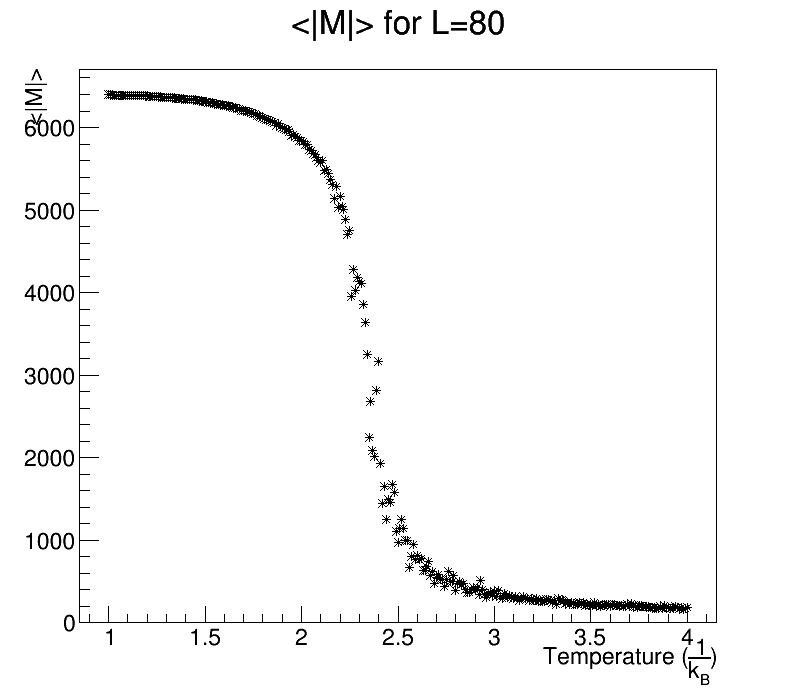
\includegraphics[width=0.3\textwidth]{plots/parte/expAbsM_latsize80}
} \\
\subfigure[]{
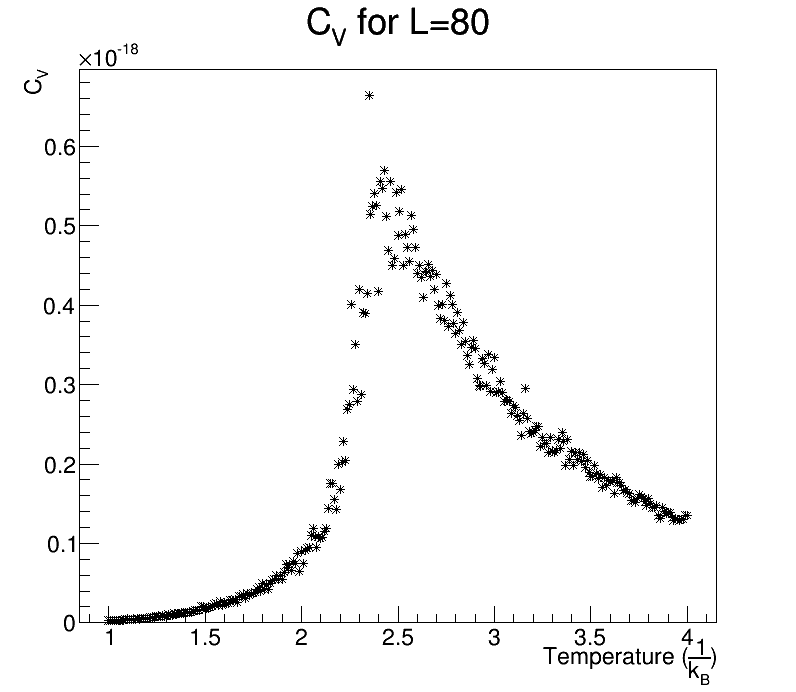
\includegraphics[width=0.3\textwidth]{plots/parte/CV_latsize80}
}
\subfigure[]{
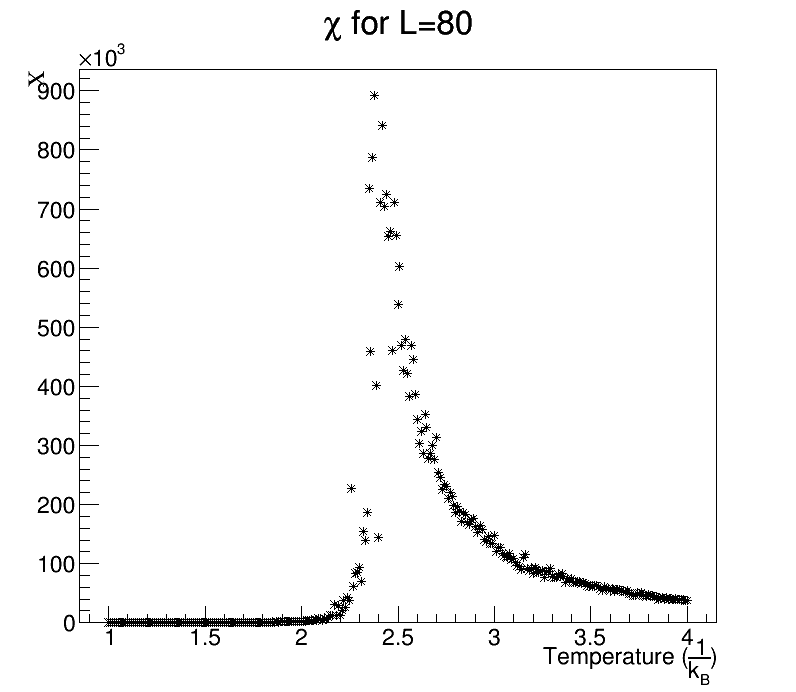
\includegraphics[width=0.3\textwidth]{plots/parte/susceptibility_latsize80}
}
\caption{Statistical quantities for a $80\times80$ lattice with a steady initial state plotted against the temperature.}
\label{fig:latsize80}
\end{center}
\end{figure}

\begin{figure}[h]
\begin{center}
\subfigure[]{
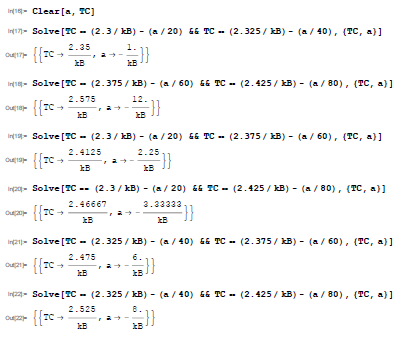
\includegraphics[width=0.6\textwidth]{solveTC1}
}
\caption{Using Mathematica~\textbf{need citation} to solve for the possible values of $T_{C}(L=\infty)$ given the data from Table~\ref{tab:tcl} and~\eqref{eq:tcscale}.}
\label{fig:tcsolve}
\end{center}
\end{figure}

\subsection{Testing Random Number Generators}
\label{subsec:randosresults}

As discussed in Section~\ref{subsec:benchmarks}, we are interested particularly in looking at the effect of random number generators on our results, looking particularly at \texttt{ran0}, \texttt{ran1}, \texttt{ran2}, \texttt{ran3}, and \texttt{rand()}, the standard C++ random number generator, with which all of the data in Section~\ref{sec:results} was created.  Overall, we find that the choice of random number generator didn't have major contributions to the results determined.  However, small differences were observed.\footnote{Throughout this discussion, we are working with the generation of a $2\times2$ lattice with an initial random configuration at a temperature of $T=1/k_{B}$.}  For example, it was observed that, if we plotted the number of accepted MC against the total number of MC cycles used in the calculation, the slopes were slightly different.   In particular, \texttt{ran1}, \texttt{ran3}, and \texttt{rand()} have more accepted MC than do \texttt{ran0} or \texttt{ran2}.  
\par But what is really important is whether or not changing the random number generator would effect the physics.  As an example, see Fig.~\ref{fig:randoschi}, where we have plotted the magnetic susceptibility $\chi$ as a function of the total number of MC cycles.  Recall from Section~\ref{sec:results} that it appeared that $\chi$ was the most unstable of the statistical quantities being observed.  In fact, it does appear that the variation -- or the number of MC cycles needed to get to the equilibrium value -- may depend on the random number generator used.  In particular, the more random the generator (according the number of tests passed as discussed in Section~\ref{subsec:benchmarks} and the significance of the associated $\chi^{2}$ tests), the more MC cycles were required before the susceptibility approached a constant value.  Still, regardless of the random number generator used, the final value of $\chi$ was the same.  
\par Because no effect was more pronounced than that on $\chi$, we assume that it is safe to use any of the five random number generators tested.  It is expected, however, that, as the number of MC cycles increases, this will no longer be true.  This is because the period of the random number generators will eventually play a roll in the calculations, which is an undesired result (at that point the numbers can be considered correlated and thus, by definition, no longer random).  Statistical biases in the form of patterns may begin to creep up in the data when the number of MC cycles nears the period of the random number generator being used, and so it is important to find a generator with a remarkably long period (such as the Mersenne Twister, which has a period of roughly $2^{19937}$~\textbf{lecture}).

\begin{figure}[h]
\begin{center}
\subfigure[]{
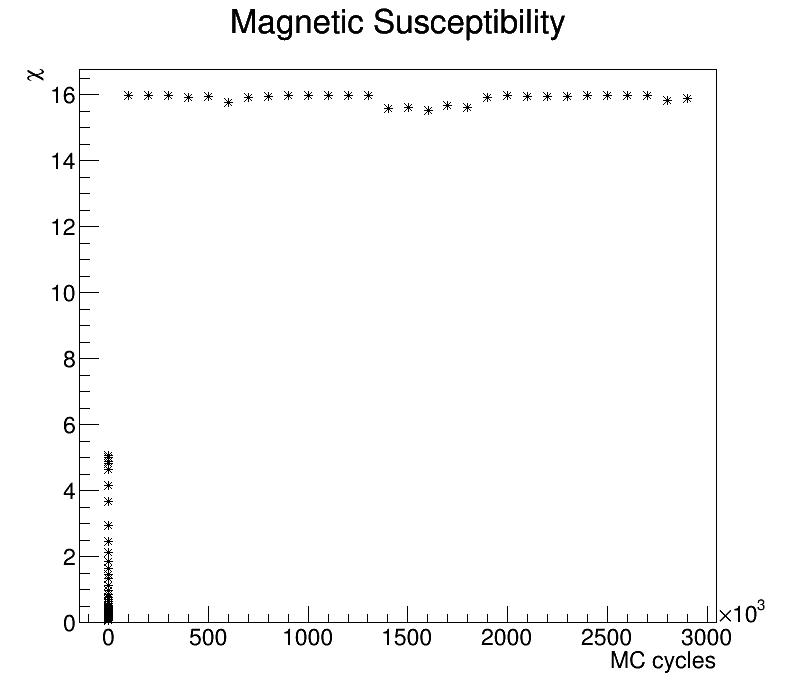
\includegraphics[width=0.3\textwidth]{benchmarks/ran0/plots_random_chi_size2_temp1}
}
\subfigure[]{
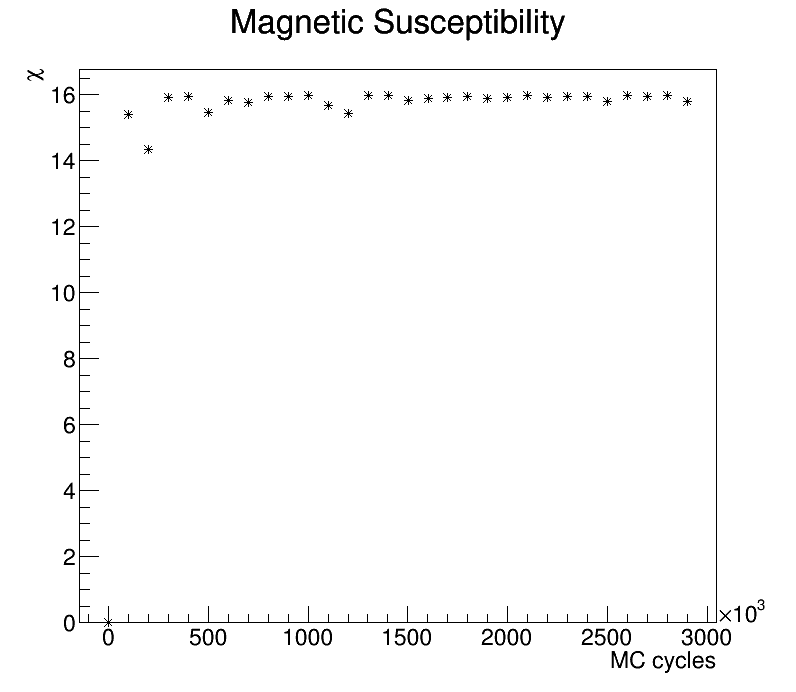
\includegraphics[width=0.3\textwidth]{benchmarks/ran1/plots_random_chi_size2_temp1}
} \\
\subfigure[]{
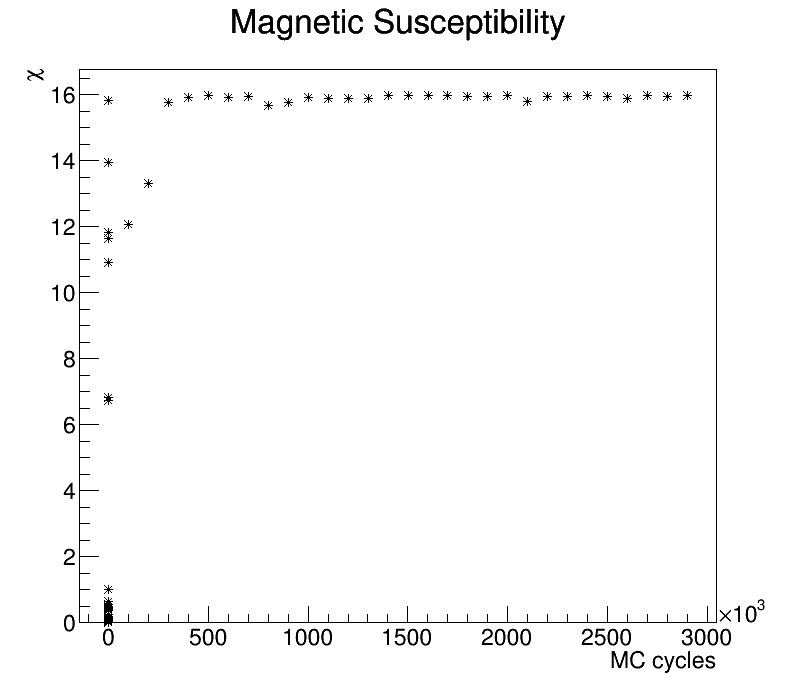
\includegraphics[width=0.3\textwidth]{benchmarks/ran2/plots_random_chi_size2_temp1}
}
\subfigure[]{
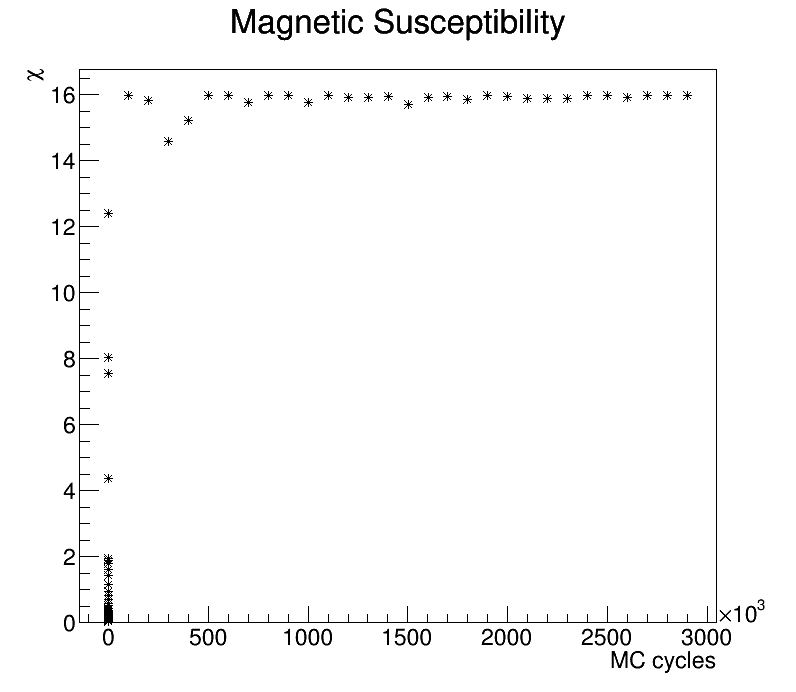
\includegraphics[width=0.3\textwidth]{benchmarks/ran3/plots_random_chi_size2_temp1}
} \\
\subfigure[]{
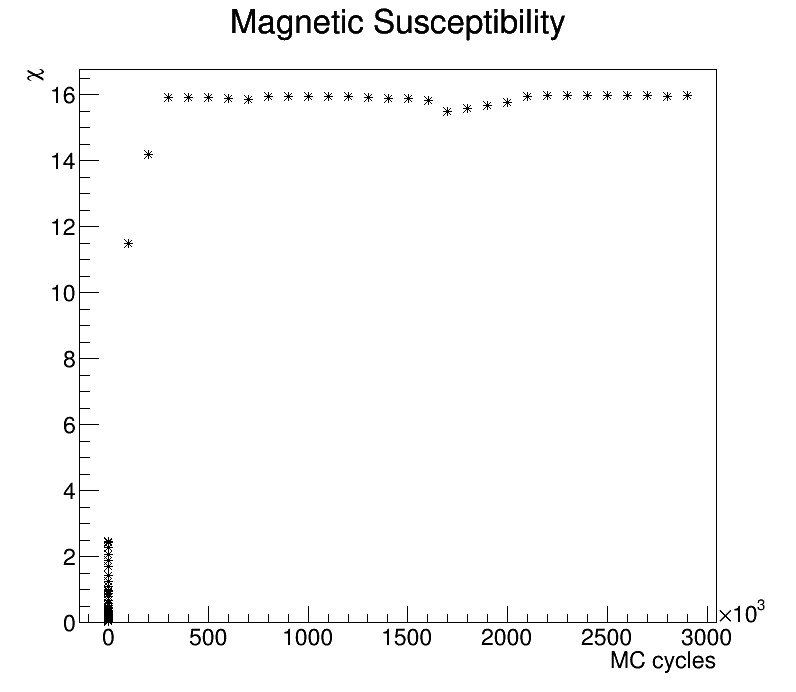
\includegraphics[width=0.3\textwidth]{benchmarks/plots/plots_random_chi_size2_temp1}
}
\caption{Magnetic susceptibility $\chi$ as a function of the number of MC cycles used in the calculation for (a) \texttt{ran0}, (b) \texttt{ran1}, (c) \texttt{ran2}, (d) \texttt{ran3}, and (e) \texttt{rand()}.}
\label{fig:randoschi}
\end{center}
\end{figure}

\section{Conclusions}
\label{sec:conc}

The Ising model in two dimensions is an immensely useful tool in statistical mechanics as a means by which to calculate expected values (such as that of the energy and magnetization), as well as fundamental properties of matter (such as the heat capacity and magnetic susceptibility).  From these quantities, it is possible to determine the critical temperature, $T_{C}$, at which phase transitions occur.  We were able (see Section~\ref{sec:results}) to do this calculation for an infinite lattice to within $14\%$ accuracy by estimating the $T_{C}$ from plots generated of $\chi$ and $C_{V}$ of various sized lattices.
\par In addition to its physical importance, the Ising model proves to be an excellent introduction to Monte Carlo generation.  We were able to develop a code to implement Monte Carlo under the guise of the Metropolis Algorithm~\textbf{need citation; also make sure I mentioned this somewhere earlier} within a new \texttt{lattice} class, which performed the calculations of our various important statistical mechanical quantities for us.  Because random number generation is key in any Monte Carlo simulation, we were also able to run some benchmark tests on five common random number generators to ensure that they were, indeed, random, and that the physics produced was not effected by the random number generator chosen.
\par \textbf{in conclusion...}



\end{document}
